\documentclass{article}

\usepackage[english]{babel}
\usepackage{amsthm,amsmath,lipsum}
\usepackage[algo2e]{algorithm2e} 
\usepackage{xcolor}
\usepackage{fullpage}
\usepackage{amssymb}
\usepackage{centernot}
%\usepackage{authblk}
\usepackage{tikz}
\usepackage{soul}
\usetikzlibrary{shapes.geometric, arrows}
\usetikzlibrary{positioning}
\usetikzlibrary{calc}


\DeclareFontFamily{U}{mathb}{\hyphenchar\font45}
\DeclareFontShape{U}{mathb}{m}{n}{
      <5> <6> <7> <8> <9> <10> gen * mathb
      <10.95> mathb10 <12> <14.4> <17.28> <20.74> <24.88> mathb12
}{}
\DeclareSymbolFont{mathb}{U}{mathb}{m}{n}
\DeclareMathSymbol{\llcurly}{3}{mathb}{"CE}
\DeclareMathSymbol{\ggcurly}{3}{mathb}{"CF}


\usepackage{thm-restate}




\theoremstyle{plain}

\newtheorem{example}{Example}
\newtheorem{theorem}{Theorem}
\newtheorem{lemma}{Lemma}
\newtheorem{definition}{Definition}
\newtheorem{observation}{Observation}
\newtheorem{corollary}{Corollary}
\newtheorem{claim}{Claim}


\usepackage{times}
\usepackage{soul}
\usepackage{url}
\usepackage[hidelinks]{hyperref}
\usepackage[utf8]{inputenc}
\usepackage[small]{caption}
\usepackage{graphicx}
\usepackage{amsmath}
\usepackage{amsthm}
\usepackage{amssymb}
\usepackage{booktabs}
\usepackage{booktabs}
\usepackage{algorithm}
\usepackage{algorithmic}
\usepackage{color}
\usepackage[switch]{lineno}

\urlstyle{same}
\usepackage[most]{tcolorbox}










\title{Maximin Share Guarantees for Few Agents with Subadditive Valuations}



\author{George Christodoulou\thanks{Aristotle University of
    Thessaloniki, and Archimedes/Athena RC, Greece. Email: \texttt{\{gichristo,vgchrist,smastra\}@csd.auth.gr} }
\and{Vasilis Christoforidis\footnotemark[1]}
\and {Symeon Mastrakoulis\footnotemark[1]}
\and Alkmini Sgouritsa\thanks{Athens University of Economics and Business, and Archimedes/Athena RC, Greece. Email: \texttt{alkmini@aueb.gr}}}

%\affil[1]{Aristotle University of
 %   Thessaloniki and Archimedes/Athena RC, Greece.}  
%\affil[2]{Athens University of Economics and Business, and Archimedes/Athena RC, Greece.}
\date{}



\begin{document}

\maketitle

\begin{abstract}
    We study the problem of fairly allocating a set of indivisible items among a set of agents. We consider the notion of (approximate) maximin share (MMS) and we provide an improved lower bound of $1/2$ (which is tight) for the case of subadditive valuations when the number of agents is at most four. We also provide a tight lower bound for the case of multiple agents, when they are equipped with one of two possible types of valuations. Moreover, we propose a new model that extends previously studied models in the area of fair division, which will hopefully give rise to further research. We demonstrate the usefulness of this model by employing it as a technical tool to derive our main result, and we provide a thorough analysis for this model for the case of three agents. Finally, we provide an improved impossibility result for the case of three submodular agents. 
    
\end{abstract}
\usetikzlibrary {patterns,patterns.meta}
\section{Introduction}

Large language models (LLMs) have achieved remarkable success in automated math problem solving, particularly through code-generation capabilities integrated with proof assistants~\citep{lean,isabelle,POT,autoformalization,MATH}. Although LLMs excel at generating solution steps and correct answers in algebra and calculus~\citep{math_solving}, their unimodal nature limits performance in plane geometry, where solution depends on both diagram and text~\citep{math_solving}. 

Specialized vision-language models (VLMs) have accordingly been developed for plane geometry problem solving (PGPS)~\citep{geoqa,unigeo,intergps,pgps,GOLD,LANS,geox}. Yet, it remains unclear whether these models genuinely leverage diagrams or rely almost exclusively on textual features. This ambiguity arises because existing PGPS datasets typically embed sufficient geometric details within problem statements, potentially making the vision encoder unnecessary~\citep{GOLD}. \cref{fig:pgps_examples} illustrates example questions from GeoQA and PGPS9K, where solutions can be derived without referencing the diagrams.

\begin{figure}
    \centering
    \begin{subfigure}[t]{.49\linewidth}
        \centering
        \includegraphics[width=\linewidth]{latex/figures/images/geoqa_example.pdf}
        \caption{GeoQA}
        \label{fig:geoqa_example}
    \end{subfigure}
    \begin{subfigure}[t]{.48\linewidth}
        \centering
        \includegraphics[width=\linewidth]{latex/figures/images/pgps_example.pdf}
        \caption{PGPS9K}
        \label{fig:pgps9k_example}
    \end{subfigure}
    \caption{
    Examples of diagram-caption pairs and their solution steps written in formal languages from GeoQA and PGPS9k datasets. In the problem description, the visual geometric premises and numerical variables are highlighted in green and red, respectively. A significant difference in the style of the diagram and formal language can be observable. %, along with the differences in formal languages supported by the corresponding datasets.
    \label{fig:pgps_examples}
    }
\end{figure}



We propose a new benchmark created via a synthetic data engine, which systematically evaluates the ability of VLM vision encoders to recognize geometric premises. Our empirical findings reveal that previously suggested self-supervised learning (SSL) approaches, e.g., vector quantized variataional auto-encoder (VQ-VAE)~\citep{unimath} and masked auto-encoder (MAE)~\citep{scagps,geox}, and widely adopted encoders, e.g., OpenCLIP~\citep{clip} and DinoV2~\citep{dinov2}, struggle to detect geometric features such as perpendicularity and degrees. 

To this end, we propose \geoclip{}, a model pre-trained on a large corpus of synthetic diagram–caption pairs. By varying diagram styles (e.g., color, font size, resolution, line width), \geoclip{} learns robust geometric representations and outperforms prior SSL-based methods on our benchmark. Building on \geoclip{}, we introduce a few-shot domain adaptation technique that efficiently transfers the recognition ability to real-world diagrams. We further combine this domain-adapted GeoCLIP with an LLM, forming a domain-agnostic VLM for solving PGPS tasks in MathVerse~\citep{mathverse}. 
%To accommodate diverse diagram styles and solution formats, we unify the solution program languages across multiple PGPS datasets, ensuring comprehensive evaluation. 

In our experiments on MathVerse~\citep{mathverse}, which encompasses diverse plane geometry tasks and diagram styles, our VLM with a domain-adapted \geoclip{} consistently outperforms both task-specific PGPS models and generalist VLMs. 
% In particular, it achieves higher accuracy on tasks requiring geometric-feature recognition, even when critical numerical measurements are moved from text to diagrams. 
Ablation studies confirm the effectiveness of our domain adaptation strategy, showing improvements in optical character recognition (OCR)-based tasks and robust diagram embeddings across different styles. 
% By unifying the solution program languages of existing datasets and incorporating OCR capability, we enable a single VLM, named \geovlm{}, to handle a broad class of plane geometry problems.

% Contributions
We summarize the contributions as follows:
We propose a novel benchmark for systematically assessing how well vision encoders recognize geometric premises in plane geometry diagrams~(\cref{sec:visual_feature}); We introduce \geoclip{}, a vision encoder capable of accurately detecting visual geometric premises~(\cref{sec:geoclip}), and a few-shot domain adaptation technique that efficiently transfers this capability across different diagram styles (\cref{sec:domain_adaptation});
We show that our VLM, incorporating domain-adapted GeoCLIP, surpasses existing specialized PGPS VLMs and generalist VLMs on the MathVerse benchmark~(\cref{sec:experiments}) and effectively interprets diverse diagram styles~(\cref{sec:abl}).

\iffalse
\begin{itemize}
    \item We propose a novel benchmark for systematically assessing how well vision encoders recognize geometric premises, e.g., perpendicularity and angle measures, in plane geometry diagrams.
	\item We introduce \geoclip{}, a vision encoder capable of accurately detecting visual geometric premises, and a few-shot domain adaptation technique that efficiently transfers this capability across different diagram styles.
	\item We show that our final VLM, incorporating GeoCLIP-DA, effectively interprets diverse diagram styles and achieves state-of-the-art performance on the MathVerse benchmark, surpassing existing specialized PGPS models and generalist VLM models.
\end{itemize}
\fi

\iffalse

Large language models (LLMs) have made significant strides in automated math word problem solving. In particular, their code-generation capabilities combined with proof assistants~\citep{lean,isabelle} help minimize computational errors~\citep{POT}, improve solution precision~\citep{autoformalization}, and offer rigorous feedback and evaluation~\citep{MATH}. Although LLMs excel in generating solution steps and correct answers for algebra and calculus~\citep{math_solving}, their uni-modal nature limits performance in domains like plane geometry, where both diagrams and text are vital.

Plane geometry problem solving (PGPS) tasks typically include diagrams and textual descriptions, requiring solvers to interpret premises from both sources. To facilitate automated solutions for these problems, several studies have introduced formal languages tailored for plane geometry to represent solution steps as a program with training datasets composed of diagrams, textual descriptions, and solution programs~\citep{geoqa,unigeo,intergps,pgps}. Building on these datasets, a number of PGPS specialized vision-language models (VLMs) have been developed so far~\citep{GOLD, LANS, geox}.

Most existing VLMs, however, fail to use diagrams when solving geometry problems. Well-known PGPS datasets such as GeoQA~\citep{geoqa}, UniGeo~\citep{unigeo}, and PGPS9K~\citep{pgps}, can be solved without accessing diagrams, as their problem descriptions often contain all geometric information. \cref{fig:pgps_examples} shows an example from GeoQA and PGPS9K datasets, where one can deduce the solution steps without knowing the diagrams. 
As a result, models trained on these datasets rely almost exclusively on textual information, leaving the vision encoder under-utilized~\citep{GOLD}. 
Consequently, the VLMs trained on these datasets cannot solve the plane geometry problem when necessary geometric properties or relations are excluded from the problem statement.

Some studies seek to enhance the recognition of geometric premises from a diagram by directly predicting the premises from the diagram~\citep{GOLD, intergps} or as an auxiliary task for vision encoders~\citep{geoqa,geoqa-plus}. However, these approaches remain highly domain-specific because the labels for training are difficult to obtain, thus limiting generalization across different domains. While self-supervised learning (SSL) methods that depend exclusively on geometric diagrams, e.g., vector quantized variational auto-encoder (VQ-VAE)~\citep{unimath} and masked auto-encoder (MAE)~\citep{scagps,geox}, have also been explored, the effectiveness of the SSL approaches on recognizing geometric features has not been thoroughly investigated.

We introduce a benchmark constructed with a synthetic data engine to evaluate the effectiveness of SSL approaches in recognizing geometric premises from diagrams. Our empirical results with the proposed benchmark show that the vision encoders trained with SSL methods fail to capture visual \geofeat{}s such as perpendicularity between two lines and angle measure.
Furthermore, we find that the pre-trained vision encoders often used in general-purpose VLMs, e.g., OpenCLIP~\citep{clip} and DinoV2~\citep{dinov2}, fail to recognize geometric premises from diagrams.

To improve the vision encoder for PGPS, we propose \geoclip{}, a model trained with a massive amount of diagram-caption pairs.
Since the amount of diagram-caption pairs in existing benchmarks is often limited, we develop a plane diagram generator that can randomly sample plane geometry problems with the help of existing proof assistant~\citep{alphageometry}.
To make \geoclip{} robust against different styles, we vary the visual properties of diagrams, such as color, font size, resolution, and line width.
We show that \geoclip{} performs better than the other SSL approaches and commonly used vision encoders on the newly proposed benchmark.

Another major challenge in PGPS is developing a domain-agnostic VLM capable of handling multiple PGPS benchmarks. As shown in \cref{fig:pgps_examples}, the main difficulties arise from variations in diagram styles. 
To address the issue, we propose a few-shot domain adaptation technique for \geoclip{} which transfers its visual \geofeat{} perception from the synthetic diagrams to the real-world diagrams efficiently. 

We study the efficacy of the domain adapted \geoclip{} on PGPS when equipped with the language model. To be specific, we compare the VLM with the previous PGPS models on MathVerse~\citep{mathverse}, which is designed to evaluate both the PGPS and visual \geofeat{} perception performance on various domains.
While previous PGPS models are inapplicable to certain types of MathVerse problems, we modify the prediction target and unify the solution program languages of the existing PGPS training data to make our VLM applicable to all types of MathVerse problems.
Results on MathVerse demonstrate that our VLM more effectively integrates diagrammatic information and remains robust under conditions of various diagram styles.

\begin{itemize}
    \item We propose a benchmark to measure the visual \geofeat{} recognition performance of different vision encoders.
    % \item \sh{We introduce geometric CLIP (\geoclip{} and train the VLM equipped with \geoclip{} to predict both solution steps and the numerical measurements of the problem.}
    \item We introduce \geoclip{}, a vision encoder which can accurately recognize visual \geofeat{}s and a few-shot domain adaptation technique which can transfer such ability to different domains efficiently. 
    % \item \sh{We develop our final PGPS model, \geovlm{}, by adapting \geoclip{} to different domains and training with unified languages of solution program data.}
    % We develop a domain-agnostic VLM, namely \geovlm{}, by applying a simple yet effective domain adaptation method to \geoclip{} and training on the refined training data.
    \item We demonstrate our VLM equipped with GeoCLIP-DA effectively interprets diverse diagram styles, achieving superior performance on MathVerse compared to the existing PGPS models.
\end{itemize}

\fi 


 \subsection{Our contribution}

We study the existence of approximate MMS allocations, a predominant notion of fairness in settings with indivisible goods, under submodular
and subadditive valuations. We focus on settings with few agents. We are able to show the following results.

\begin{itemize}
    \item In our main technical result (Theorem~\ref{thm:mainTheorem}), we show the existence of $1/2$-MMS allocations for at most four agents with subadditive valuations. We note that this result improves the best known bounds for many other valuation classes, including OXS, Gross Substitutes, submodular and XOS. We emphasize that the guarantee of our theorem matches the best known impossibility result due to \cite{GhodsiHSSY22}, thus settling the case of four agents for both subbaditive and XOS valuations (see also Table~\ref{table:Results}). 

    \item We show the existence of $1/2$-MMS allocations for multiple agents when they have one of two admissible valuation functions (Theorem~\ref{thm:two-types}).

    
    \item On the way to prove Theorem~\ref{thm:mainTheorem} we develop a new model that is useful for inductive arguments. This model incorporates nicely previously studied MMS variants, and we believe that it is of independent interest. In Section~\ref{sec:Reductions}, we provide a thorough study of approximate guarantees for three agents and we are able to provide two complete characterizations: one for the case of $1/2$-MMS$(\mathbf{d})$ (Theorem~\ref{thm:three-general}) and one for the case of $(1,1/2,1/2)$-MMS$(\bf d)$ (Theorem~\ref{thm:three-general-approximate}). 

    \item We show an improved impossibility result for three agents with submodular valuation functions: we present an instance in which an $\alpha$-MMS allocation does not exist for $\alpha > 2/3$ (Theorem~\ref{thm:SubmodUB}). This improves the previous best known result of 3/4 due to \cite{GhodsiHSSY22}.

    
\end{itemize}




 % \vspace{-0.2cm}
\section{System Overview}
The mmE-Loc enhances the mmWave radar with an event camera to achieve accurate and low-latency drone ground localization, allowing the drone to rapidly adjust its location state and perform a precise landing.
% Given the paramount importance of safety in commercial drone operations, mmE-Loc can collaborate with RTK or visual markers to ensure precise landings.
Given the critical importance of safety in commercial drone operations, mmE-Loc can work in conjunction with RTK or visual markers to ensure precise landing performance.
In this section, we mathematically introduce the problem that mmE-Loc tries to address and provide an overview of the system design.

% mmE-Loc leverages the integration of mmWave radar and event camera data to achieve accurate, low-latency drone ground localization, allowing the drone to quickly adjust its position and perform precise landings. Given the critical importance of safety in commercial drone operations, mmE-Loc can also work in conjunction with RTK or visual markers to ensure precise landing performance.

% enabling a reliable and accurate localization service for drones (\fig \ref{overview}).

\vspace{-0.3cm}
\subsection{Problem Formulation}
In this section, we illustrate key variables in mmE-Loc and introduce the system's inputs and outputs.

% \begin{figure}[t]
%     \setlength{\abovecaptionskip}{-0.1cm} % height above Figure X caption
%     \setlength{\belowcaptionskip}{-0.3cm}
%     \setlength{\subfigcapskip}{-0.25cm}
%     \centering
%         \includegraphics[width=1\columnwidth]{Figs/reference.png}
%         \vspace{-0.2cm}
%     \caption{Illustration of reference systems and essential variables in mmE-Loc.}
%     \label{reference}
%     % \vspace{-0.6cm}
% \end{figure} 

\textbf{Reference systems.} \label{3.2}
% As shown in \fig \ref{reference}, t
There are four reference (\aka, coordinate) systems in mmE-Loc: 
$(i)$ the Event camera reference system $\mathtt{E}$; 
$(ii)$ the Radar reference system $\mathtt{R}$; 
$(iii)$ the Object reference system $\mathtt{O}$;
$(iv)$ the Drone reference system $\mathtt{D}$.
Note that a drone can be considered as an object.
For clarity, before an object is identified as a drone, we utilize $\mathtt{O}$. 
Once confirmed as a drone, we use $\mathtt{D}$ for the drone and continue using $\mathtt{O}$ for other objects.
Throughout the operation of system, $\mathtt{E}$ and $\mathtt{R}$ remain stationary and are rigidly attached together, while $\mathtt{O}$ and $\mathtt{D}$ undergo changes in accordance with movement of the object and the drone, respectively. 
The transformation from $\mathtt{R}$ to $\mathtt{E}$ can be readily obtained from calibration \cite{wang2023vital}. 

\textbf{Goal of mmE-Loc.}
The goal of mmE-Loc is to determine 3D location of the drone, defined as $t_{\mathtt{ED}}$, the translation from coordinate system $\mathtt{D}$ to $\mathtt{E}$.
Specifically, mmE-Loc optimizes and reports 3D location of drone $(l_x, l_y, l_z)$ at each timestamp $i$ with input from event stream and radar sample.
% where $t^i_{\mathtt{ED}}$ represents the translation vector from $\mathtt{D}$ to $\mathtt{E}^3$. 
$t_{\mathtt{ED}}$ and ($l_x$, $l_y$, $l_z$) are equivalent representations of the drone’s location and can be inter-converted with Rodrigues’ formula \cite{min2021joint}. 
The former representation is adopted in the paper, as it is commonly used in drone flight control systems.

\begin{figure*}[t]
    \setlength{\abovecaptionskip}{0.3cm} % height above Figure X caption
    \setlength{\belowcaptionskip}{-0.2cm}
    \setlength{\subfigcapskip}{-0.25cm}
    \centering
        \includegraphics[width=1.85\columnwidth]{Figs/trackingmodel.png}
        \vspace{-0.3cm}
    \caption{Illustration of tracking models in Consistency-instructed Collaborative Tracking algorithm.}
    \label{CCT}
    \vspace{-0.2cm}
\end{figure*} 

% We first briefly describe and illustrate some essential variables in mmE-Loc and the problem of localizing the landing drone,which is the 3D location ($l_x$, $l_y$, $l_z$).
% \todo{As shown in \fig )}, there are three reference (\aka, coordinate) systems in mmE-Loc: $(i)$ the Event camera reference system \mathtt{E}; $(ii)$ the Radar reference system \mathtt{R}; $(iii)$ the Drone reference system \mathtt{D}.


% \subsection{mmE-Loc: System goals}
% \noindent $\bullet$ \textbf{How to detect and track the drones from noisy sensing results at a high frequency?}
% Environmental changes often introduce irrelevant information in the sensing results from the event camera and mmWave radar, hindering the system's ability to identify signals changes caused by the drones to be tracked. 
% Additionally, modern flight control loops operate at frequencies exceeding 400 Hz, requiring the system to detect and track drones rapidly. 
% However, traditional noise filtering, object detection and tracking algorithms have high time complexities, resulting in precision and tracking frequency bottlenecks. 
% \todo{Explanation in figures or tables.}

% \noindent $\bullet$ \textbf{How to fuse two types of heterogeneous data to precisely localize drones at a high frequency?} 
% Once the drone is detected, accurate 3D spatial localization of it is essential, which is more time-consuming than detection and tracking due to additional processing. 
% Moreover, event cameras provide asynchronous event streams, while mmWave radar generates sparse point clouds with relatively low spatial resolution. 
% Previous fusion methods (\eg extended Kalman filters and particle filters) often suffer from significant cumulative drift error and lengthy processing times, rendering them inadequate for high-frequency and high-precision tracking.
% \todo{Explanation in figures or tables.}

\vspace{-0.3cm}
\subsection{Overview}
% mmE-Loc is a localization system designed for high-frequency and precise localization of drones, enabling them to rapidly adjust their location state and achieve accurate landing. 
As illustrated in \fig \ref{overview}, mmE-Loc comprises two key modules: 
% $(i)$ \textit{CCT} (\textbf{C}onsistency-instructed \textbf{C}ollaborative \textbf{T}racking) for noise filtering and drone detection and 
% $(ii)$ \textit{GAO} (\textbf{G}raph-informed \textbf{A}daptive \textbf{O}ptimization) for localization of drones from the integrated event stream and mmWave 3D point cloud. \todo{Fix the figure.}

\noindent $\bullet$ 
The \textit{CCT} (\textbf{C}onsistency-instructed \textbf{C}ollaborative \textbf{T}racking) for noise filtering, drone detection, and preliminary localization of the drone.
This module utilizes time-synchronized event streams and mmWave radar measurements as inputs. 
Subsequently, the \textit{Radar Tracking Model} processes radar measurements to generate a sparse 3D point cloud. 
Meanwhile, the \textit{Event Tracking Model} takes into the stream of asynchronous events for event filtering, drone detection, and tracking. 
% Finally, \textit{Consistency-instructed Measurements Filter} aligns the results of the both tracking models leverage the consistency between both modalities, and then utilizes periodic micro motion of drone to extract drone-related measurements,  eliminate noise and error detections, and roughly localize the drone.
Finally, \textit{Consistency-instructed Measurements Filter} aligns the outputs of both tracking models by leveraging \textit{temporal-consistency} between the two modalities. 
It then utilizes the drone's periodic micro-motion to extract drone-specific measurements and achieve drone preliminary localization.

\noindent $\bullet$
The \textit{GAJO} (\textbf{G}raph-informed \textbf{A}daptive \textbf{J}oint \textbf{O}ptimization) for fine localization and trajectory optimization of the drone.
% GAJO initially derives preliminary estimates of drone motion and location, using radar measurements and event camera tracking results, respectively. 
% GAJO includes a carefully designed \textit{factor graph-based optimization} method, which 通过深入挖掘事件相机与radar的潜力, jointly fuses and refines the outputs from both the \textit{Event Tracking Model} and \textit{Radar Tracking Model} to accurately determine the location of drone. 
Based on the operational principles of two sensors and their respective noise distributions, \textit{GAJO} incorporates a meticulously designed \textit{factor graph-based optimization} method. 
This module employs the \textit{spatial-complementarity} from both modalities to unleash the potential of event camera and mmWave radar in drone ground localization.
Specifically, \textit{GAJO} jointly fuses the preliminary location estimation from the \textit{Event Tracking Model} and the \textit{Radar Tracking Model} and adaptively refines them, determining the fine location of drone with $ms$-level processing time.
% Finally, to expedite the process of the \textit{factor graph-based location optimization} method, we transform factor graph into a Bayes tree through elimination and optimize the drone's location adaptively via a \textit{Incremental Optimization method}. 

 \section{Related Works}
\label{sec:rw}

%-------------------------------------------------------------------------
\noindent \textbf{Vision-Language Model.}
In recent years, vision-language models, as a novel tool capable of processing both visual and linguistic modalities, have garnered widespread attention. These models, such as CLIP~\cite{clip}, ALIGN~\cite{ALIGN}, BLIP~\cite{BLIP}, FILIP~\cite{filip}, etc., leverage self-supervised training on image-text pairs to establish connections between vision and text, enabling the models to comprehend image semantics and their corresponding textual descriptions. This powerful understanding allows vision-language models (e.g., CLIP) to exhibit remarkable generalization capabilities across various downstream tasks~\cite{downsteam1,downsteam2,downsteam3,h2b}. To further enhance the transferability of vision-language models to downstream tasks, prompt tuning and adapter methods have been applied. However, methods based on prompt tuning (such as CoOp~\cite{coop}, CoCoOp~\cite{cocoop}, Maple~\cite{maple}) and adapter-based methods (such as Tip-Adapter~\cite{tip}, CLIP-Adapter~\cite{clip_adapter}) often require large amounts of training data when transferring to downstream tasks, which conflicts with the need for rapid adaptation in real-world applications. Therefore, this paper focuses on test-time adaptation~\cite{tpt}, a method that enables transfer to downstream tasks without relying on training data.

%-------------------------------------------------------------------------
\noindent \textbf{Test-Time Adaptation.}
Test-time adaptation~(TTA) refers to the process by which a model quickly adapts to test data that exhibits distributional shifts~\cite{tta1,memo,ptta,domainadaptor,dota}. Specifically, it requires the model to handle these shifts in downstream tasks without access to training data. TPT~\cite{tpt} optimizes adaptive text prompts using the principle of entropy minimization, ensuring that the model produces consistent predictions for different augmentations of test images generated by AugMix~\cite{augmix}. DiffTPT~\cite{difftpt} builds on TPT by introducing the Stable Diffusion Model~\cite{stable} to create more diverse augmentations and filters these views based on their cosine similarity to the original image. However, both TPT and DiffTPT still rely on backpropagation to optimize text prompts, which limits their ability to meet the need for fast adaptation during test-time. TDA~\cite{tda}, on the other hand, introduces a cache model like Tip-Adapter~\cite{tip} that stores representative test samples. By comparing incoming test samples with those in the cache, TDA refines the model’s predictions without the need for backpropagation, allowing for test-time enhancement. Although TDA has made significant improvements in the TTA task, it still does not fundamentally address the impact of test data distribution shifts on the model and remains within the scope of CLIP's original feature space. We believe that in TTA tasks, instead of making decisions in the original space, it would be more effective to map the features to a different spherical space to achieve a better decision boundary.

%-------------------------------------------------------------------------
\noindent \textbf{Statistical Learning.}
Statistical learning techniques play an important role in dimensionality reduction and feature extraction. Support Vector Machines~(SVM)~\cite{svm} are primarily used for classification tasks but have been adapted for space mapping through their ability to create hyperplanes that separate data in high-dimensional spaces. The kernel trick enables SVM to operate in transformed feature spaces, effectively mapping non-linearly separable data. PCA~\cite{pca} is a linear transformation method that maps high-dimensional data to a new lower-dimensional space through a linear transformation, while preserving as much important information from the original data as possible.

 \section{Preliminaries}\label{subs:preliminaries}

For a comprehensive introduction to feedback linearization, the interested reader is referred to \cite{Isidori1995}.

Consider a multivariable nonlinear system
    \begin{equation}
    \left\{
\begin{split}
     \dot{\xv}&= \fv(\xv)+\Gm(\xv)\uv,\\
    \yv &= \hv(\xv),
    \label{eq:sys}
    \end{split}
    \right.
    \end{equation}
where \mbox{$\xv\in \mathbb{R}^n$} is the state, the input matrix is \mbox{$\Gm(\xv)=\begin{bmatrix}
    \gv_1(\xv)  \;\cdots \; \gv_{p}(\xv)
\end{bmatrix}\in \mathbb{R}^{n \times p}$}, $\fv(\xv)$,  $\gv_1(\xv), \ldots, \gv_{p}(\xv)$ are smooth vector fields, and $\hv(\xv)=\begin{bmatrix} h_1(\xv)  \cdots h_{p}(\xv)\end{bmatrix}^\top$ is a smooth function defined on an open set of $\mathbb{R}^n$.
The  system (\ref{eq:sys}) is said to have \emph{(vector) relative degree} $\rv = \{
    r_1, \ldots, r_{p}
\}$ at a point $\xv^\circ$ w.r.t. the input-output pair  $(\uv,\yv)$ if  
\begin{flalign}
&\text{\textrm{(i)}}    & L_{\gv_j}L^{k}_{\fv} h_i(\xv) &=0,&
\end{flalign}
for all $1\leq j \leq p$, for all $k\leq r_i-1$, for all $1\leq i \leq p$ and for all $\xv$ in a neighborhood of $\xv^\circ$, and\\
\textrm{(ii)}\;\;  the $p\times p$ matrix 
   \begin{align}
    \Am(\xv) &:= 
         \begin{pmatrix}
            L_{\gv_1}L^{r_1-1}_{\fv}h_1(\xv) & \cdots&  L_{\gv_{p}}L^{r_1-1}_{\fv}h_1(\xv) \\ 
            L_{\gv_1}L^{r_2-1}_{\fv}h_2(\xv) & \cdots&  L_{\gv_{p}}L^{r_2-1}_{\fv}h_2(\xv) \\  
            \vdots & & \vdots \\
            L_{\gv_1}L^{r_{p}-1}_{\fv}h_{p}(\xv) & \cdots&  L_{\gv_{p}}L^{r_{p}-1}_{\fv}h_{p}(\xv) 
        \end{pmatrix}
    \label{eq:intbmatrix}
\end{align}  
is nonsingular at $\xv = \xv^\circ$. 
The output array at the $\rv$-th derivative may then be written as an affine system of the form
\begin{equation}
{\yv}^{(\rv)} :=\begin{bmatrix}
    y_1^{(r_1)} \;\cdots\;  y_{p}^{(r_{p})}
\end{bmatrix}^\top =\bv(\xv)+\Am(\xv)\uv,
\label{eq:y_r_now}
\end{equation}
with 
\begin{equation}
 \bv(\xv):=\begin{bmatrix}
L_{\boldsymbol{f}}^{(r_1)}{h_1(\xv)} \; \cdots \; 
L_{\boldsymbol{f}}^{(r_{p})}{h_{p}(\xv)}
\end{bmatrix}^\top.
\label{eq:b}
\end{equation}


Suppose the system \eqref{eq:sys} has some \emph{(vector) relative degree} $\rv:=\{r_1,\ldots,r_p\}$ at $\xv^\circ$ and that the matrix $\Gm(\xv^\circ)$ has rank $p$ in a  neighborhood $\mathcal{U}$ of $\xv^\circ$. Suppose also that  \mbox{$r_1+r_2+\ldots+r_p=n$}, and choose the  control input to be $$\uv = \Am^{-1}(\xv)[-\bv(\xv)+\vv],
$$
where $\vv \in \mathbb{R}^{p}$ can be assigned freely and $\Am(\xv), \bv(\xv)$ are defined as in~(\ref{eq:intbmatrix}) and~(\ref{eq:b}).
Then the output dynamics \eqref{eq:y_r_now} become
$$
\yv^{(\rv)} = \vv.
$$
We refer to \(\yv\) as a \textit{linearizing output array}, which possesses the property that the entire state and input of the system can be expressed in terms of \(\yv\) and its time derivatives. 



 \section{Subadditive Valuations}
\label{sec:SubaddVal}

In this section we present our main technical result which establishes the existence of $1/2$-MMS allocation for the case of at most four agents (Theorem~\ref{thm:mainTheorem}). In Sections~\ref{sec:2Subadd}-~\ref{sec:4Subadd} we establish the existence of $1/2$-MMS approximate allocations for two, three and four subadditive agents (Corollaries~\ref{cor:2agents},~\ref{cor:3agents}~and~\ref{cor:4agents}), respectively, that follow as simple corollaries from more restricted settings (Lemmas~\ref{Lemma:2agents}, \ref{Lemma:threehalfs}, and \ref{Lemma:4agents}, respectively). We note that all these results improve the state-of-the-art for MMS guarantees for a wide set of valuation classes that lie below subadditive in the complement-free hierarchy. Subsequently, in Section \ref{sec:MoreAgents} we show how our proof techniques can be extended to obtain positive results for settings with many agents, when the agents have one of two types of admissible valuation functions. We emphasize that all the results presented herein are tight for subadditive valuations, i.e., there exist constructions where not all agents can receive more than $1/2$ of their MMS values \cite{GhodsiHSSY22}. In the proofs which follow we use ``symmetric'' cuts, i.e. no matter if $\mathcal{X}^*_i(C)=\mathcal{X}_i(C)$ or $\mathcal{X}^*_i(C)=\mathcal{X}_i(M \setminus C)$ for the maximum desired half of agent $i$ over cut $C$, the proof will continue the same way. 


\begin{theorem}
\label{thm:mainTheorem}
    An $1/2$-MMS allocation exists for at most four agents with subadditive valuations.
\end{theorem}

Before proceeding with the proofs for few agents, we give the following general observation that illustrates the implications of our results. 

\begin{observation}
\label{obs:simpleReduction}
    Given some fair division instance, an allocation that is $\boldsymbol{\alpha}$-MMS$(\mathbf{d})$ is also $\boldsymbol{\alpha}'$-MMS$(\mathbf{d}')$, where $\boldsymbol{\alpha}$ is pointwise larger or equal to $\boldsymbol{\alpha}'$, and $\mathbf{d}$ is pointwise smaller or equal to $\mathbf{d}'$.
\end{observation}
\begin{proof}
    Let $A=(A_1,\ldots, A_n)$ be a $\boldsymbol{\alpha}$-MMS$(\mathbf{d})$ allocation. By definition it holds that for each agent $i$, $v_i(A_i)\geq \alpha_i \mu_i^{d_i}$. 
    
    We first show that $A$ is also a $\boldsymbol{\alpha}$-MMS$(\mathbf{d}')$ allocation.  
    Note that if for some agent $i$ there exists a partition of $M$ into $d_i'$ bundles that she values each by at least $\mu_i^{d_i'}$, then there exists a partition into $d_i\le d_i'$ bundles that she values by at least the same amount, by merging bundles of the first partition, due to monotonicity of the valuation functions. This in turns implies that $\mu_i^{d_i}\geq \mu_i^{d_i'}$. Therefore, $v_i(A_i)\geq \alpha_i \mu_i^{d_i'}$, for all $i$, which implies that $A$ is a $\boldsymbol{\alpha}$-MMS$(\mathbf{d}')$ allocation. 
    
    To complete the proof, it simply holds that $v_i(A_i)\geq \alpha_i \mu_i^{d_i'}\ge \alpha_i' \mu_i^{d_i'}$, for all $i$, which means that $A$ is also a $\boldsymbol{\alpha}'$-MMS$(\mathbf{d}')$ allocation. 
\end{proof}


\subsection{Two Agents}
\label{sec:2Subadd}
In this section we show that there always exists a $1/2$-MMS allocation for the case of two agents. We first show a stronger statement (Lemma~\ref{Lemma:2agents}) and obtain the main result as a corollary (Corollary~\ref{cor:2agents}). We further provide a useful restatement (Corollary~\ref{Cor:cut-and-choose}) of Lemma~\ref{Lemma:2agents} to be extensively used in the proofs for three and four agents.

\begin{lemma}[Two agents]
\label{Lemma:2agents}
    A $(1/2,1)$-MMS$(1,2)$ allocation exists for two agents with subadditive valuation functions. 
\end{lemma}


\begin{proof}


    We denote by $S$ and $T$ the two agents and by $S_j, T_j$ their $j$-th MMS bundle respectively, i.e., $S_1$ for the first agent and $T_1, T_2$ for the second agent. 
    We proceed in a cut-and-choose fashion; we partition the set of items into two disjoint bundles $T_1, T_2$ which both are worth at least $1$ for $T$. Agent $S$ picks her favorite bundle which (due to subadditivity) is guaranteed to have at least $1/2$ value since $v_S(T_1) + v_S(T_2) \geq v_S(T_1 \cup T_2)=v_S(S_1)= 1$, and $T$ receives the remaining bundle. Hence a $(1/2,1)$-MMS$(1,2)$ allocation exists (see Figure \ref{fig:2agentsRed} for an illustration).
\end{proof}

In the following corollary we state that Lemma~\ref{Lemma:2agents} suggests that a $1/2$-MMS approximation is attainable for two agents (by Observation~\ref{obs:simpleReduction}); this bound is tight for two agents \cite{GhodsiHSSY22}. 

\begin{corollary}
\label{cor:2agents}
    A $1/2$-MMS allocation exists for two agents with subadditive valuation functions.
\end{corollary}

\begin{center}
%
\begin{figure}
\begin{center}
    \begin{tabular}{ccc}
%
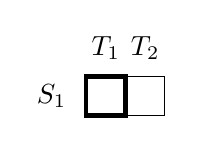
\begin{tikzpicture}[scale=0.5]
  \draw[step=1cm,] (0,0) grid (2,1);
  %\fill[black!20](0,0) rectangle +(1,1);
  \draw[black, ultra thick](0,0) rectangle +(1,1);
\node[anchor=north] at (0.5,2.25) {$T_1$};
\node[anchor=north] at (1.5,2.25) {$T_2$};
\node[anchor=west] at (-1.5,0.5) {$S_1$};
\end{tikzpicture}
& 
\begin{tikzpicture}[scale=0.5]
  \draw[step=1cm,] (0,0) grid (2,1);

(1,0) rectangle +(1,1);
\draw[pattern={north west lines},pattern color=red]
(1,0) rectangle +(1,1);
\draw[pattern={horizontal lines},pattern color=blue](0,0) rectangle (1,1);
\node[anchor=north] at (0.5,2.25) {$T_1$};
\node[anchor=north] at (1.5,2.25) {$T_2$};
\node[anchor=west] at (-1.5,0.5) {$S_1$};
\end{tikzpicture} 
& 
\begin{tikzpicture}[scale=0.5]
  \draw[step=1cm,] (0,0) grid (2,1);
\draw[pattern={north west lines},pattern color=red](0,0) rectangle (1,1);
\draw[pattern={horizontal lines},pattern color=blue](1,0) rectangle +(1,1);
\node[anchor=north] at (0.5,2.25) {$T_1$};
\node[anchor=north] at (1.5,2.25) {$T_2$};
\node[anchor=west] at (-1.5,0.5) {$S_1$};
\end{tikzpicture}\\
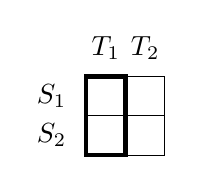
\begin{tikzpicture}[scale=0.5]

%\draw[pattern={north west lines},pattern color=blue](0,0) rectangle +(1,2);
\draw[black, ultra thick](0,0) rectangle +(1,2);
%\draw[pattern={horizontal lines},pattern color=red](1,0) rectangle (2,2);
%\draw[pattern={horizontal lines},pattern color=blue](1,0) rectangle (2,2);
  \draw[step=1cm,] (0,0) grid (2,2);

\node[anchor=north] at (0.5,3.25) {$T_1$};
\node[anchor=north] at (1.5,3.25) {$T_2$};
\node[anchor=west] at (-1.5,1.5) {$S_1$};
\node[anchor=west] at (-1.5,0.5) {$S_2$};
\end{tikzpicture} & \begin{tikzpicture}[scale=0.5]

(0,1) rectangle +(1,1);
\draw[pattern={horizontal lines},pattern color=blue]
(0,1) rectangle +(1,1);
;
\draw[pattern={north west lines},pattern color=red](1,0) rectangle (2,2);
  \draw[step=1cm,] (0,0) grid (2,2);

\node[anchor=north] at (0.5,3.25) {$T_1$};
\node[anchor=north] at (1.5,3.25) {$T_2$};
\node[anchor=west] at (-1.5,1.5) {$S_1$};
\node[anchor=west] at (-1.5,0.5) {$S_2$};
\end{tikzpicture} &
\begin{tikzpicture}[scale=0.5]
(0,0) rectangle +(1,2);
\draw[pattern={north west lines},pattern color=red]
(0,0) rectangle +(1,2);
\draw[pattern={horizontal lines},pattern color=blue](1,1) rectangle +(1,1);
  \draw[step=1cm,] (0,0) grid (2,2);

\node[anchor=north] at (0.5,3.25) {$T_1$};
\node[anchor=north] at (1.5,3.25) {$T_2$};
\node[anchor=west] at (-1.5,1.5) {$S_1$};
\node[anchor=west] at (-1.5,0.5) {$S_2$};
\end{tikzpicture}\\
(a)&(b)&(c)\\

    \end{tabular}
    \end{center}
        \caption{We illustrate the partition for both $\boldsymbol{d}=(1,2)$ and $\boldsymbol{d}=(2,2)$. The set of items $S_1$ can be divided into $T_1$ and $T_2$. If agent $S$ values bundle $T_1 \cap S_1$ (represented with a thick line in (a)) more than $\frac{v_S(S_1)}{2}$ then allocation (b) has the desired properties (the blue bundle for agent $S$ and the red bundle for agent $T$). If this is not the case, then due to the subadditivity, the same holds for agent $S$ and bundle $T_2 \cap S_1$; then (b) has the desired properties.} 
    \label{fig:2agentsRed}
\end{figure}
\end{center}
We also provide a useful restatement of Lemma~\ref{Lemma:2agents} to be used as a reduction tool in the proofs with more agents.
\begin{corollary}
\label{Cor:cut-and-choose}
    Consider a fair division instance of two agents with subadditive valuations and a set of $M$ items, where one agent values $M$ at least $1$, and there exists a partition into two bundles where the other agent values each at least $1/2$. Then, there exists an allocation that guarantees at least $1/2$ value to each agent.
\end{corollary}



\subsection{Three Agents}
\label{sec:3Subadd}
In this section we show that there exists a $1/2$-MMS allocation for the case of three agents. Again, we first show a stronger statement (Lemma~\ref{Lemma:threehalfs}) and obtain the main result as a corollary (Corollary~\ref{cor:3agents}). 

\begin{lemma} [Three agents]
\label{Lemma:threehalfs}
    An $1/2$-MMS$(3,2,2)$ allocation exists for three agents with subadditive valuation functions.
\end{lemma}
\begin{proof}
We denote by $S,T,Q$ the three agents and by $S_j,T_j,Q_j$ their $j$-th MMS bundle, respectively. 

The proof relies on the existence of $(1/2,1)$-MMS$(1,2)$ in the instance with two agents; we show that we can identify a valuable subset $A_T$ (with value at least $1/2$) to allocate to agent $T$, such that we can extend the allocation applying Corollary \ref{Cor:cut-and-choose} for agents $S$ and $Q$ and for the remaining items $M\setminus A_T$. In particular, agent $Q$ will have value at least $1$ for $M\setminus A_T$, while agent $S$ will be able to partition it into two bundles with value at least $1/2$ each. To achieve this we will use two cuts sequentially, first to agent $S$ and then (based on the response of $S$) to agent $T$  (we refer the reader to Figure~\ref{fig:3agents} (a) for an illustration of the proof).
    
{\bf First cut.} Consider the cut $C=T_2$ that we offer to $S$ and let $S_1^*,S_2^* \in \mathcal{X}_{S}^*(C)$ be two bundles in the maximum desired half (by Observation~\ref{obs:Cut_noOfDesiredSets} there exist at least two such bundles). The cut is ``symmetric'' for $T$ in a sense that both $C=T_2$ and $M\setminus C=T_1$ contain the {\em same number of $T$'s MMS bundles}; so it is without loss of generality to assume that $\mathcal{X}^*_S(C)=\mathcal{X}_S(C)$ (in Figure~\ref{fig:3agents} (a) $S_1^* \subseteq S_1,S_2^* \subseteq S_2$ are represented with blue color).

{\bf Second cut.} We next offer $C=Q_1$ to $T$ and let  $T_1^* \in \mathcal{X}_T^*(C)$ be the bundle in the maximum desired half. The cut is ``symmetric'' for $Q$, so again without loss of generality assume that $\mathcal{X}_T^*(C)=\mathcal{X}_T(C)$ (in Figure~\ref{fig:3agents} (b) $T_1^* \subseteq T_1$ is represented with red color).

    
{\bf Apply Corollary \ref{Cor:cut-and-choose}.} Overall, $v_T(T^*_1)\geq 1/2$ and $T^*_1$ will be allocated to $T$. Then, for $M'=M\setminus T^*_1$, it holds that $v_Q(M')\geq v_Q(Q_2) \geq 1$, and $S_1^*,S_2^*\subseteq M'$, for both of which $S$ has value at least $1/2$. So the lemma follows by using Corollary \ref{Cor:cut-and-choose} on $M'$ for agents $Q$ and $S$. (in Figure~\ref{fig:3agents} (c) $S_1^* \subseteq S_1,S_1^* \subseteq S_2$ are represented with blue color and $Q_2$ with green).
\end{proof}
\begin{center}

\begin{figure}
\begin{center}

\begin{tabular}{ccc}

\small{
\begin{tikzpicture}[scale=0.45]
\draw[yslant=0.5,xslant=-1,black, ultra thick](3,3) (5,1) rectangle +(-2,-1);  
\draw[yslant=0.5,black, ultra thick](3,-3) rectangle +(2,3);    \draw[yslant=-0.5,black, ultra thick](3,3) rectangle +(-1,-3); 
\draw[yslant=0.5,xslant=-1,pattern={horizontal lines},pattern color=blue] (5,1) rectangle +(-2,-1);  
\draw[yslant=0.5,pattern={horizontal lines},pattern color=blue](3,-2) rectangle +(2,2);    \draw[yslant=-0.5,pattern={horizontal lines},pattern color=blue](3,3) rectangle +(-1,-2);     

    \draw[yslant=-0.5] (1,0) grid (3,3);
  \draw[yslant=0.5] (3,-3) grid (5,0);
  \draw[yslant=0.5,xslant=-1] (3,0) grid (5,2);
\node[anchor=south west] at (-0.2,1.5,0) {$S_1$};
\node[anchor=south west] at (-0.2,0.5,0) {$S_2$};
\node[anchor=south west] at (-0.2,-0.5,0) {$S_3$};
\node[anchor=north west] at (0.45,3.7,0) {$Q_1$};
\node[anchor=north west] at (1.5,4.3,0) {$Q_2$};
\node[anchor=north west] at (0.5,-0.8,0) {$T_1$};
\node[anchor=north west] at (1.5,-1.3,0) {$T_2$};
\end{tikzpicture}} &
\small{
\begin{tikzpicture}[scale=0.45]
  
    \draw[yslant=0.5,xslant=-1,color=black,ultra thick] (4,2) rectangle +(-1,-2);
    %\fill[yslant=0.5,xslant=-1,color=black!20](4,2) rectangle +(-1,-2); 
    \draw[yslant=0.5,color=black,ultra thick] (3,-3) rectangle +(1,3);
    %\fill[yslant=0.5,color=black!20](3,-3) rectangle +(1,3);

    \draw[yslant=-0.5,color=black,ultra thick](3,3) rectangle +(-2,-3);
    %\fill[yslant=-0.5,color=black!20](3,3) rectangle +(-2,-3);
    
    \draw[yslant=0.5,xslant=-1,pattern={north west lines},pattern color=red](4,2) rectangle +(-1,-1);
\draw[yslant=-0.5,pattern={north west lines},pattern color=red](2,3) rectangle +(-1,-3);
  \draw[yslant=-0.5] (1,0) grid (3,3);
  \draw[yslant=0.5] (3,-3) grid (5,0);
  \draw[yslant=0.5,xslant=-1] (3,0) grid (5,2);
\node[anchor=south west] at (-0.2,1.5,0) {$S_1$};
\node[anchor=south west] at (-0.2,0.5,0) {$S_2$};
\node[anchor=south west] at (-0.2,-0.5,0) {$S_3$};
\node[anchor=north west] at (0.45,3.7,0) {$Q_1$};
\node[anchor=north west] at (1.5,4.3,0) {$Q_2$};
\node[anchor=north west] at (0.5,-0.8,0) {$T_1$};
\node[anchor=north west] at (1.5,-1.3,0) {$T_2$};
\end{tikzpicture}} &
\small{
\begin{tikzpicture}[scale=0.45]
 \draw[yslant=0.5,xslant=-1,pattern={north west lines},pattern color=red](4,2) rectangle +(-1,-1);
\draw[yslant=-0.5,pattern={north west lines},pattern color=red](2,3) rectangle +(-1,-3);
\draw[yslant=0.5,xslant=-1,pattern={crosshatch dots},pattern color=green]  (5,2) rectangle +(-1,-2);
    \draw[yslant=0.5,pattern={crosshatch dots},pattern color=green]  (4,-3) rectangle +(1,3);

    \draw[yslant=0.5,xslant=-1,pattern={horizontal lines},pattern color=blue] (5,1) rectangle +(-2,-1);
    \draw[yslant=0.5,pattern={horizontal lines},pattern color=blue](3,-2) rectangle +(2,2);
    \draw[yslant=-0.5,pattern={horizontal lines},pattern color=blue](3,3) rectangle (2,1);
  \draw[yslant=-0.5] (1,0) grid (3,3);
  \draw[yslant=0.5] (3,-3) grid (5,0);
  \draw[yslant=0.5,xslant=-1] (3,0) grid (5,2);
\node[anchor=south west] at (-0.2,1.5,0) {$S_1$};
\node[anchor=south west] at (-0.2,0.5,0) {$S_2$};
\node[anchor=south west] at (-0.2,-0.5,0) {$S_3$};
\node[anchor=north west] at (0.45,3.7,0) {$Q_1$};
\node[anchor=north west] at (1.5,4.3,0) {$Q_2$};
\node[anchor=north west] at (0.5,-0.8,0) {$T_1$};
\node[anchor=north west] at (1.5,-1.3,0) {$T_2$};
\end{tikzpicture}}\\
(a) & (b) & (c) \\
$S_1^*,S_2^* \in \mathcal{X}_S^*(T_2)$ &  $T_1^* \in \mathcal{X}^*_T(Q_1)$ & Apply Corollary \ref{Cor:cut-and-choose}\\
\end{tabular}
    
\end{center}
\caption{We use blue, red, and green to denote the bundles from which we will allocate to agents $S,T$ and $Q$, respectively. The thickened lines illustrate the first and second cuts, while (c) demonstrates the application of Corollary 2.
}
\label{fig:3agents}
\end{figure} 
\end{center}
As a corollary of Lemma~\ref{Lemma:threehalfs}, a $1/2$-MMS allocation always exists for three agents (by Observation~\ref{obs:simpleReduction}); this bound is also tight \cite{GhodsiHSSY22}. 
\begin{corollary}
\label{cor:3agents}
    A $1/2$-MMS allocation exists for three agents with subadditive valuation functions. 
\end{corollary}


\subsection{Four Agents}
In this section we show the existence of $1/2$-MMS allocation for the case of four agents, our main technical result. We are also able to show a stronger statement (Lemma~\ref{Lemma:4agents}) and obtain the main result as a corollary (Corollary~\ref{cor:4agents}). 

\label{sec:4Subadd}

\begin{lemma} [Four agents]
\label{Lemma:4agents}
    A $1/2$-MMS$(3,3,4,4)$ allocation exists for four agents with subadditive valuation functions.
\end{lemma}
\begin{proof}
    We denote by $S,T,Q,R$ the four agents and by $S_j,T_j,Q_j,R_j$ their $j$-th MMS bundle, respectively. 
    
    We progressively identify four candidate allocations in total, and we show that one of those should be a $1/2$-MMS$(3,3,4,4)$ allocation. 

    In a nutshell, the protocol works as follows. By offering carefully chosen cuts to agents $S,T,Q$ we are able to find partial allocations for two of those agents (in the first round these are $S$ and $T$), that have high enough value (higher than $1/2$), in a way that always preserves one MMS bundle of agent $R$ {\em intact}, let it be $R_4$. If the third agent (this is $Q$ in the first round) values higher than $1/2$ two of her bundles (on the remaining items) then we can apply Corollary~\ref{Cor:cut-and-choose} on $Q$ and $R$ and for the remaining items, and we can claim a $1/2$-MMS$(3,3,4,4)$ allocation. If this is not the case, then the third agent must value at least two of the intersections of her bundles with the partial allocation of the other two agents with value higher than $1/2$. In the next round we will tentatively allocate to the third agent one of these sets. We will also keep one of the other two agents and offer her a subset of high value {\em from a different bundle} (the notion of maximum desired half is useful to achieve this last property). We proceed in a similar manner by querying the remaining agent investigating again whether Corollary~\ref{Cor:cut-and-choose} can be employed. The key is that in every round that the third agent does not satisfy the conditions of Corollary~\ref{Cor:cut-and-choose} we are able to build a more structured partial allocation, which in the final step provides an allocation of $M\setminus R_4$ to agents $S,T$ and $Q$, that they value by at least $1/2$. Then $R_4$ can be allocated to agent $R$ and the allocation is $1/2$-MMS$(3,3,4,4)$.
    
\begin{center}

\begin{figure}[t]
\begin{center}

    \begin{tabular}{cc}
\small{
\begin{tikzpicture}[scale=0.425]
\draw[yslant=0.5,ultra thick, black](4,-3) rectangle +(4,1);     
\draw[yslant=-0.5,ultra thick, black](4,2) rectangle +(-3,-1); 
\draw[yslant=-0.5,pattern={north west lines},pattern color=red](4,3) rectangle +(-1,-1);
\draw[yslant=-0.5,pattern={north west lines},pattern color=red](4,1) rectangle +(-1,-1);
\draw[yslant=0.5,xslant=-1,pattern={north west lines},pattern color=red](7,0) rectangle +(-4,-1); 
\draw[yslant=0.5,pattern={north west lines},pattern color=red](4,-2) rectangle +(4,1);   
\draw[yslant=0.5,pattern={north west lines},pattern color=red](4,-4) rectangle +(4,1);   
%\draw[yslant=0.5,xslant=-1,pattern={horizontal lines},pattern color=blue](7,2) rectangle +(-4,-3);  
\draw[yslant=0.5,pattern={horizontal lines},pattern color=blue](4,-3) rectangle +(4,1);     
\draw[yslant=-0.5,pattern={horizontal lines},pattern color=blue](4,2) rectangle +(-3,-1);     
  \draw[yslant=-0.5] (1,0) grid (4,3);
  \draw[yslant=0.5] (4,-4) grid (8,-1);
  \draw[yslant=0.5,xslant=-1] (3,-1) grid (7,2);
\node[anchor=south west] at (-0.25,1.5,0) {$S_1$};
\node[anchor=south west] at (-0.25,0.5,0) {$S_2$};
\node[anchor=south west] at (-0.25,-0.5,0) {$S_3$};
\node[anchor=north west] at (0.5,3.8,0) {$Q_1$};
\node[anchor=north west] at (1.5,4.3,0) {$Q_2$};
\node[anchor=north west] at (2.5,4.8,0) {$Q_3$};
\node[anchor=north west] at (3.5,5.3,0) {$Q_4$};
\node[anchor=north west] at (0.4,-0.8,0) {$T_3$};
\node[anchor=north west] at (1.4,-1.3,0) {$T_2$};
\node[anchor=north west] at (2.4,-1.8,0) {$T_1$};
\node[anchor=north] at (7,5,0) {$R_1$};
\end{tikzpicture}}
&
\small{
\begin{tikzpicture}[scale=0.425]
\draw[yslant=0.5,ultra thick, black](4,-3) rectangle +(4,1);     
\draw[yslant=-0.5,ultra thick, black](4,2) rectangle +(-3,-1); 
\draw[yslant=-0.5,pattern={north west lines},pattern color=red](4,3) rectangle +(-1,-1);
\draw[yslant=-0.5,pattern={north west lines},pattern color=red](4,1) rectangle +(-1,-1);
\draw[yslant=0.5,xslant=-1,pattern={north west lines},pattern color=red](7,0) rectangle +(-4,-1); 
\draw[yslant=0.5,pattern={north west lines},pattern color=red](4,-2) rectangle +(4,1);   
\draw[yslant=0.5,pattern={north west lines},pattern color=red](4,-4) rectangle +(4,1);   
%\draw[yslant=0.5,xslant=-1,pattern={horizontal lines},pattern color=blue](7,2) rectangle +(-4,-3);  
\draw[yslant=0.5,pattern={horizontal lines},pattern color=blue](4,-3) rectangle +(4,1);     
\draw[yslant=-0.5,pattern={horizontal lines},pattern color=blue](4,2) rectangle +(-3,-1);      
  \draw[yslant=-0.5] (1,0) grid (4,3);
  \draw[yslant=0.5] (4,-4) grid (8,-1);
  \draw[yslant=0.5,xslant=-1] (3,-1) grid (7,2);
\node[anchor=south west] at (-0.25,1.5,0) {$S_1$};
\node[anchor=south west] at (-0.25,0.5,0) {$S_2$};
\node[anchor=south west] at (-0.25,-0.5,0) {$S_3$};
\node[anchor=north west] at (0.5,3.8,0) {$Q_1$};
\node[anchor=north west] at (1.5,4.3,0) {$Q_2$};
\node[anchor=north west] at (2.5,4.8,0) {$Q_3$};
\node[anchor=north west] at (3.5,5.3,0) {$Q_4$};
\node[anchor=north west] at (0.4,-0.8,0) {$T_3$};
\node[anchor=north west] at (1.4,-1.3,0) {$T_2$};
\node[anchor=north west] at (2.4,-1.8,0) {$T_1$};
\node[anchor=north] at (7,5,0) {$R_2$};
\end{tikzpicture}}\\
\small{
\begin{tikzpicture}[scale=0.425]
\draw[yslant=-0.5,pattern={north west lines},pattern color=red](4,3) rectangle +(-1,-3);
\draw[yslant=0.5,xslant=-1,pattern={north west lines},pattern color=red](7,0) rectangle +(-4,-1); 
\draw[yslant=0.5,pattern={north west lines},pattern color=red](4,-4) rectangle +(4,3);    
  \draw[yslant=-0.5] (1,0) grid (4,3);
  \draw[yslant=0.5] (4,-4) grid (8,-1);
  \draw[yslant=0.5,xslant=-1] (3,-1) grid (7,2);
\node[anchor=south west] at (-0.25,1.5,0) {$S_1$};
\node[anchor=south west] at (-0.25,0.5,0) {$S_2$};
\node[anchor=south west] at (-0.25,-0.5,0) {$S_3$};
\node[anchor=north west] at (0.5,3.8,0) {$Q_1$};
\node[anchor=north west] at (1.5,4.3,0) {$Q_2$};
\node[anchor=north west] at (2.5,4.8,0) {$Q_3$};
\node[anchor=north west] at (3.5,5.3,0) {$Q_4$};
\node[anchor=north west] at (0.4,-0.8,0) {$T_3$};
\node[anchor=north west] at (1.4,-1.3,0) {$T_2$};
\node[anchor=north west] at (2.4,-1.8,0) {$T_1$};
\node[anchor=north] at (7,5,0) {$R_3$};
\end{tikzpicture}}
&

\small{
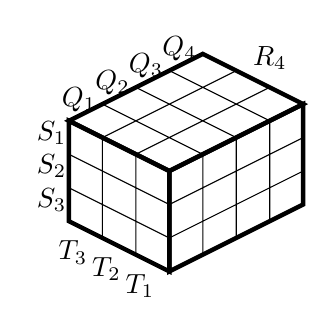
\begin{tikzpicture}[scale=0.425]
\draw[yslant=0.5,ultra thick, black](4,-4) rectangle +(4,3);     
\draw[yslant=-0.5,ultra thick, black](4,3) rectangle +(-3,-3); 
\draw[yslant=0.5,xslant=-1,ultra thick, black](7,2) rectangle +(-4,-3);    
  \draw[yslant=-0.5] (1,0) grid (4,3);
  \draw[yslant=0.5] (4,-4) grid (8,-1);
  \draw[yslant=0.5,xslant=-1] (3,-1) grid (7,2);
\node[anchor=south west] at (-0.25,1.5,0) {$S_1$};
\node[anchor=south west] at (-0.25,0.5,0) {$S_2$};
\node[anchor=south west] at (-0.25,-0.5,0) {$S_3$};
\node[anchor=north west] at (0.5,3.8,0) {$Q_1$};
\node[anchor=north west] at (1.5,4.3,0) {$Q_2$};
\node[anchor=north west] at (2.5,4.8,0) {$Q_3$};
\node[anchor=north west] at (3.5,5.3,0) {$Q_4$};
\node[anchor=north west] at (0.4,-0.8,0) {$T_3$};
\node[anchor=north west] at (1.4,-1.3,0) {$T_2$};
\node[anchor=north west] at (2.4,-1.8,0) {$T_1$};
\node[anchor=north] at (7,5,0) {$R_4$};
\end{tikzpicture}}\\
\end{tabular}
    
\end{center}
\caption{The first candidate allocation $A=(S_2^*,T_1^*)$ for four agents and $\boldsymbol{d}=(3,3,4,4)$. We use blue to denote $S_2^* \subseteq S_2$ and red to denote $T_1^* \subseteq T_1$. We use a thick line to illustrate the cut $C=\{S^*_2 \cup R_4\}$. The allocation is valid and none of the bundles intersects with $R_4$. The cuts are symmetric, i.e. if we had $\mathcal{X}_S^*(C) =\mathcal{X}_S^*(M\setminus C)$ for cut $C=\{R_1 \cup R_2\}$ or/and $\mathcal{X}_T^*(C)=\mathcal{X}_T(C)$ for the corresponding cut $C$, we could construct the same allocation by renaming the bundles.}
\label{fig:4agents1}
\end{figure}
\end{center}



    
  
    
    \noindent{\bf Building the first candidate allocation}. We first consider agent $S$ (an agent with $3$ MMS bundles) and cut her MMS bundles by offering the cut $C=R_1 \cup R_2$. By Observation~\ref{obs:Cut_noOfDesiredSets} there are at least two bundles in the set $\mathcal{X}_{S}^*(C)$; let those be $S_1^*,S_2^* \in \mathcal{X}_{S}^*(C)$. We note that $S_1^*,S_2^*$ intersect with exactly two MMS bundles of $R$, so w.l.o.g. assume that those are $R_1,R_2$, i.e., assume that $\mathcal{X}_{S}^*(C)=\mathcal{X}_{S}(C)$. Therefore
     \begin{equation}
        \label{eq:4agentsCond0}
        S_j^*\cap R_3 = \emptyset \mbox{ and } S_j^*\cap R_4 = \emptyset, \mbox{ for } j \in \{1,2\}\,.
    \end{equation}
    

    Next, we offer a cut to agent $T$ in a way that a) ensures that a {\em whole} MMS bundle of agent $R$ remains intact and b) one of $S_1^*, S_2^*$ does not intersect with the Maximum Desired Half of $T$. A cut that serves this purpose is $C=S_2^* \cup R_4$. Now each of the sets $C$ and $M\setminus C$ intersects with exactly one of $S^*_1, S^*_2$ and with exactly one of $R_3, R_4$ which are the remaining whole bundles of $R$. W.l.o.g. assume that $\mathcal{X}_{T}^*(C)=\mathcal{X}_{T}(M \setminus C)$.\footnote{Even if it is w.l.o.g., we consider $\mathcal{X}_{T}^*(C)=\mathcal{X}_{T}(M \setminus C)$ that includes $S_3$ to avoid any confusion of the steps needed, because the case of $\mathcal{X}_{T}^*(C)=\mathcal{X}_{T}(C)$ is simpler and can be handled the same way.} 
    By Observation~\ref{obs:Cut_noOfDesiredSets} there are at least two bundles in the set $\mathcal{X}_{T}^*(C)$, let those be $T_1^*,T_2^* \in \mathcal{X}_{T}^*(C)$. Then, it holds that 
    \begin{equation}
    \label{eq:4agentsCond1}
        T_j^*\cap R_4 = \emptyset \mbox{ and } T_j^*\cap S_2^* = \emptyset, \mbox{ for } j \in \{1,2\}\,.
    \end{equation}
    
    {\bf First candidate allocation.} Consider the following partial allocation for $S$ and $T$: $A= (S^*_2,T^*_1)$ (see Figure \ref{fig:4agents1} for an illustration). By construction, both $S$ and $T$ value their allocated bundles by at least $1/2$. If there exist at least two MMS bundles of $Q$ that she values with at least $1/2$ {\em after the removal of $S^*_2\cup T^*_1$}, then the conditions of Corollary~\ref{Cor:cut-and-choose} are satisfied for $Q$ and $R$ for the remaining items (recall that $R$ values the remaining items by at least $1$ since they contain $R_4$). Hence by  employing Corollary~\ref{Cor:cut-and-choose} we can find an allocation of $M\setminus (S^*_2\cup T^*_1)$ to $Q$ and $R$ where they both value their bundles with at least $1/2$, and we are done.   
        
    So, suppose that this is not the case. Then there must be at least three MMS bundles of $Q$, let them be $Q_1,Q_2,Q_3$, such that $v_Q(Q_j\cap(S^*_2\cup T^*_1))\geq 1/2$ for $j\in\{1, 2, 3\}$. In other words, if we consider the cut $C=S^*_2\cup T^*_1$ for agent $Q$, then it is guaranteed that $Q_1^*,Q^*_2,Q^*_3 \in \mathcal{X}_{Q}(C)$. Since $Q_j^*\subseteq S^*_2\cup T^*_1$, for all $j \in \{1,2,3\}$ and also by \eqref{eq:4agentsCond0} and \eqref{eq:4agentsCond1} we conclude that
    \begin{equation}
        \label{eq:4agentsCond2}
        Q_j^* \cap T^*_2 = \emptyset \mbox{ and } Q_j^* \cap R_4= \emptyset , \mbox{ for } j \in \{1,2,3\}\,.
    \end{equation}


    \begin{figure}[h] 
\begin{center}
    \begin{tabular}{cc}
\small{
\begin{tikzpicture}[scale=0.425]
\draw[yslant=-0.5,ultra thick, black](4,3) rectangle +(-1,-3);
\draw[yslant=0.5,xslant=-1,ultra thick, black](7,0) rectangle +(-4,-1); 
\draw[yslant=0.5,ultra thick, black](4,-4) rectangle +(4,3);   
       
\draw[yslant=-0.5,ultra thick, black](3,2) rectangle +(-2,-1);
\draw[yslant=-0.5,ultra thick, white](3,2) rectangle +(0,-1);
\draw[yslant=0.5,pattern={crosshatch dots},pattern color=green] (4,-4) rectangle +(1,3);
\draw[yslant=-0.5,pattern={crosshatch dots},pattern color=green](4,3) rectangle +(-1,-3);
\draw[yslant=-0.5,pattern={crosshatch dots},pattern color=green](3,2) rectangle +(-2,-1);
\draw[yslant=-0.5,pattern={north west lines},pattern color=red](3,3) rectangle +(-1,-1);
\draw[yslant=-0.5,pattern={north west lines},pattern color=red](3,1) rectangle +(-1,-1);
\draw[yslant=0.5,xslant=-1,pattern={north west lines},pattern color=red](7,1) rectangle +(-4,-1); 
\draw[yslant=0.5,xslant=-1,pattern={crosshatch dots},pattern color=green](4,0) rectangle +(-1,-1);     
  \draw[yslant=-0.5] (1,0) grid (4,3);
  \draw[yslant=0.5] (4,-4) grid (8,-1);
  \draw[yslant=0.5,xslant=-1] (3,-1) grid (7,2);
\node[anchor=south west] at (-0.25,1.5,0) {$S_1$};
\node[anchor=south west] at (-0.25,0.5,0) {$S_2$};
\node[anchor=south west] at (-0.25,-0.5,0) {$S_3$};
\node[anchor=north west] at (0.5,3.8,0) {$Q_1$};
\node[anchor=north west] at (1.5,4.3,0) {$Q_2$};
\node[anchor=north west] at (2.5,4.8,0) {$Q_3$};
\node[anchor=north west] at (3.5,5.3,0) {$Q_4$};
\node[anchor=north west] at (0.4,-0.8,0) {$T_3$};
\node[anchor=north west] at (1.4,-1.3,0) {$T_2$};
\node[anchor=north west] at (2.4,-1.8,0) {$T_1$};
\node[anchor=north] at (7,5,0) {$R_1$};
\end{tikzpicture}}
&
\small{
\begin{tikzpicture}[scale=0.425]
\draw[yslant=-0.5,ultra thick, black](4,3) rectangle +(-1,-3);
\draw[yslant=0.5,xslant=-1,ultra thick, black](7,0) rectangle +(-4,-1); 
\draw[yslant=0.5,ultra thick, black](4,-4) rectangle +(4,3);   
       
\draw[yslant=-0.5,ultra thick, black](3,2) rectangle +(-2,-1);
\draw[yslant=-0.5,ultra thick, white](3,2) rectangle +(0,-1);
\draw[yslant=0.5,pattern={crosshatch dots},pattern color=green] (4,-4) rectangle +(1,3);
\draw[yslant=-0.5,pattern={crosshatch dots},pattern color=green](4,3) rectangle +(-1,-3);
\draw[yslant=-0.5,pattern={crosshatch dots},pattern color=green](3,2) rectangle +(-2,-1);
\draw[yslant=-0.5,pattern={north west lines},pattern color=red](3,3) rectangle +(-1,-1);
\draw[yslant=-0.5,pattern={north west lines},pattern color=red](3,1) rectangle +(-1,-1);
\draw[yslant=0.5,xslant=-1,pattern={north west lines},pattern color=red](7,1) rectangle +(-4,-1); 
\draw[yslant=0.5,xslant=-1,pattern={crosshatch dots},pattern color=green](4,0) rectangle +(-1,-1);    
  \draw[yslant=-0.5] (1,0) grid (4,3);
  \draw[yslant=0.5] (4,-4) grid (8,-1);
  \draw[yslant=0.5,xslant=-1] (3,-1) grid (7,2);
\node[anchor=south west] at (-0.25,1.5,0) {$S_1$};
\node[anchor=south west] at (-0.25,0.5,0) {$S_2$};
\node[anchor=south west] at (-0.25,-0.5,0) {$S_3$};
\node[anchor=north west] at (0.5,3.8,0) {$Q_1$};
\node[anchor=north west] at (1.5,4.3,0) {$Q_2$};
\node[anchor=north west] at (2.5,4.8,0) {$Q_3$};
\node[anchor=north west] at (3.5,5.3,0) {$Q_4$};
\node[anchor=north west] at (0.4,-0.8,0) {$T_3$};
\node[anchor=north west] at (1.4,-1.3,0) {$T_2$};
\node[anchor=north west] at (2.4,-1.8,0) {$T_1$};
\node[anchor=north] at (7,5,0) {$R_2$};
\end{tikzpicture}}\\
\small{
\begin{tikzpicture}[scale=0.425]
\draw[yslant=-0.5,ultra thick, black](4,3) rectangle +(-1,-3);
\draw[yslant=0.5,xslant=-1,ultra thick, black](7,0) rectangle +(-4,-1); 
\draw[yslant=0.5,ultra thick, black](4,-4) rectangle +(4,3);   
       
\draw[yslant=-0.5,pattern={north west lines},pattern color=red](3,3) rectangle +(-1,-3);
\draw[yslant=0.5,xslant=-1,pattern={north west lines},pattern color=red](7,1) rectangle +(-4,-1); 
\draw[yslant=-0.5,pattern={crosshatch dots},pattern color=green](4,3) rectangle +(-1,-3);
\draw[yslant=0.5,xslant=-1,pattern={crosshatch dots},pattern color=green](4,0) rectangle +(-1,-1); 
\draw[yslant=0.5,pattern={crosshatch dots},pattern color=green](4,-4) rectangle +(1,3);    
  \draw[yslant=-0.5] (1,0) grid (4,3);
  \draw[yslant=0.5] (4,-4) grid (8,-1);
  \draw[yslant=0.5,xslant=-1] (3,-1) grid (7,2);
\node[anchor=south west] at (-0.25,1.5,0) {$S_1$};
\node[anchor=south west] at (-0.25,0.5,0) {$S_2$};
\node[anchor=south west] at (-0.25,-0.5,0) {$S_3$};
\node[anchor=north west] at (0.5,3.8,0) {$Q_1$};
\node[anchor=north west] at (1.5,4.3,0) {$Q_2$};
\node[anchor=north west] at (2.5,4.8,0) {$Q_3$};
\node[anchor=north west] at (3.5,5.3,0) {$Q_4$};
\node[anchor=north west] at (0.4,-0.8,0) {$T_3$};
\node[anchor=north west] at (1.4,-1.3,0) {$T_2$};
\node[anchor=north west] at (2.4,-1.8,0) {$T_1$};
\node[anchor=north] at (7,5,0) {$R_3$};
\end{tikzpicture}}
&

\small{
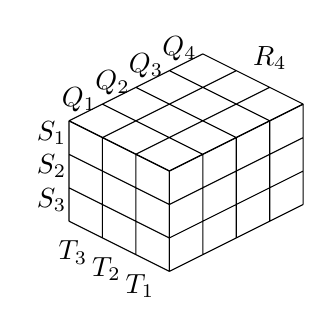
\begin{tikzpicture}[scale=0.425]

    
  \draw[yslant=-0.5] (1,0) grid (4,3);
  \draw[yslant=0.5] (4,-4) grid (8,-1);
  \draw[yslant=0.5,xslant=-1] (3,-1) grid (7,2);
\node[anchor=south west] at (-0.25,1.5,0) {$S_1$};
\node[anchor=south west] at (-0.25,0.5,0) {$S_2$};
\node[anchor=south west] at (-0.25,-0.5,0) {$S_3$};
\node[anchor=north west] at (0.5,3.8,0) {$Q_1$};
\node[anchor=north west] at (1.5,4.3,0) {$Q_2$};
\node[anchor=north west] at (2.5,4.8,0) {$Q_3$};
\node[anchor=north west] at (3.5,5.3,0) {$Q_4$};
\node[anchor=north west] at (0.4,-0.8,0) {$T_3$};
\node[anchor=north west] at (1.4,-1.3,0) {$T_2$};
\node[anchor=north west] at (2.4,-1.8,0) {$T_1$};
\node[anchor=north] at (7,5,0) {$R_4$};
\end{tikzpicture}}\\
\end{tabular}
    
\end{center}
\caption{The second candidate allocation $A'=(T_2^*,Q_1^*)$. We use red for bundle $T_2^* \subseteq T_2$ and green for $Q_1^*\subseteq Q_1$. The cut $C=\{T_1^* \cup S_2^*\}$ is shown with a thick line. We try to apply Corollary \ref{cor:2agents} for agents $S$ and $R$ and the set of items $M \setminus (T_2^*\cup Q_1^*)$. We could construct the same allocation for any $3$ bundles $Q_i^*$ by renaming the bundles.}
\label{fig:4agents2}
\end{figure}

    {\bf Second candidate allocation.} Next, we consider the partial allocation $A'= (T^*_2,Q^*_1)$ for agents $T$ and $Q$ which by (\ref{eq:4agentsCond2}) is valid and both $v_T(T^*_2), v_Q(Q_1^*)$ are higher than $1/2$ (see Figure \ref{fig:4agents2} for an illustration). If there exist at least two MMS bundles of $S$, that she values with at least $1/2$ {\em after the removal of $T^*_2 \cup Q^*_1$}, then by employing Corollary \ref{Cor:cut-and-choose} we can find an allocation of $M\setminus (T^*_2\cup Q^*_1)$ to $S$ and $R$ where they both value their bundles with at least $1/2$, and we are done.
    
    
    Otherwise, it should be that for the cut $C=T^*_2 \cup Q^*_1$  there are two sets\footnote{We note that it is not necessarily the case that $S'_1\subseteq S_1$ or $S'_2\subseteq S_2$ although this is how it is depicted in the figures for the sake of exposition.} $S_1',S_2' \in \mathcal{X}_{S}(C)$. 
    Since for any $j \in \{1,2\}$, $S_j'\subseteq T^*_2 \cup Q^*_1$, by \eqref{eq:4agentsCond1} and \eqref{eq:4agentsCond2} we conclude
    \begin{equation}
        \label{eq:4agentsCond3}
        S_j' \cap Q^*_2 = \emptyset, S_j' \cap Q^*_3 = \emptyset \mbox{ and } S_j' \cap R_4 = \emptyset, \mbox{ for } j \in \{1,2\}\,.
    \end{equation}
    
    
    {\bf Third candidate allocation.} Consider now the partial allocation $A''= (S'_1,Q^*_2)$ for $S$ and $Q$, which is valid (due to (\ref{eq:4agentsCond3})) and both agents value their allocated bundles by at least $1/2$ (see Figure \ref{fig:4agents3} for an illustration).
    Again, if there exist at least two MMS bundles of $T$, that she values with at least $1/2$ after the removal of $S'_1\cup Q^*_2$, by using Corollary \ref{Cor:cut-and-choose} on $T$ and $R$, we are done (similarly as in the previous cases). 
    
 
  

\begin{figure}[H]
\begin{center}

    \begin{tabular}{cc}
\small{
\begin{tikzpicture}[scale=0.425]
      
 
\draw[yslant=0.5,ultra thick, black] (4,-4) rectangle +(1,3);
\draw[yslant=-0.5,ultra thick, black](4,3) rectangle +(-2,-3);
\draw[yslant=-0.5,ultra thick, black](2,2) rectangle +(-1,-1);
\draw[yslant=-0.5,ultra thick, white](3,1) rectangle +(-1,1);
\draw[yslant=0.5,xslant=-1,ultra thick, black](7,1) rectangle +(-4,-1); 
\draw[yslant=0.5,xslant=-1,ultra thick, black](4,0) rectangle +(-1,-1); 
\draw[yslant=0.5,xslant=-1,ultra thick, white](3,0) rectangle +(1,0); 

\draw[yslant=0.5,pattern={crosshatch dots},pattern color=green] (5,-4) rectangle +(1,3);
\draw[yslant=0.5,xslant=-1,pattern={crosshatch dots},pattern color=green](5,0) rectangle +(-1,-1); 
\draw[yslant=0.5,pattern={horizontal lines},pattern color=blue](4,-2) rectangle +(1,1);    
\draw[yslant=0.5,xslant=-1,pattern={horizontal lines},pattern color=blue](7,1) rectangle +(-4,-1);
\draw[yslant=0.5,xslant=-1,pattern={horizontal lines},pattern color=blue](4,0) rectangle +(-1,-1);
%\draw[yslant=-0.5,pattern={horizontal lines},pattern color=blue](4,2) rectangle +(-3,-1);     
\draw[yslant=-0.5,pattern={horizontal lines},pattern color=blue](4,3) rectangle +(-2,-1);    
  \draw[yslant=-0.5] (1,0) grid (4,3);
  \draw[yslant=0.5] (4,-4) grid (8,-1);
  \draw[yslant=0.5,xslant=-1] (3,-1) grid (7,2);
\node[anchor=south west] at (-0.25,1.5,0) {$S_1$};
\node[anchor=south west] at (-0.25,0.5,0) {$S_2$};
\node[anchor=south west] at (-0.25,-0.5,0) {$S_3$};
\node[anchor=north west] at (0.5,3.8,0) {$Q_1$};
\node[anchor=north west] at (1.5,4.3,0) {$Q_2$};
\node[anchor=north west] at (2.5,4.8,0) {$Q_3$};
\node[anchor=north west] at (3.5,5.3,0) {$Q_4$};
\node[anchor=north west] at (0.4,-0.8,0) {$T_3$};
\node[anchor=north west] at (1.4,-1.3,0) {$T_2$};
\node[anchor=north west] at (2.4,-1.8,0) {$T_1$};
\node[anchor=north] at (7,5,0) {$R_1$};
\end{tikzpicture}}
&
\small{
\begin{tikzpicture}[scale=0.425]

\draw[yslant=0.5,ultra thick, black] (4,-4) rectangle +(1,3);
\draw[yslant=-0.5,ultra thick, black](4,3) rectangle +(-2,-3);
\draw[yslant=-0.5,ultra thick, black](2,2) rectangle +(-1,-1);
\draw[yslant=-0.5,ultra thick, white](3,1) rectangle +(-1,1);
\draw[yslant=0.5,xslant=-1,ultra thick, black](7,1) rectangle +(-4,-1); 
\draw[yslant=0.5,xslant=-1,ultra thick, black](4,0) rectangle +(-1,-1); 
\draw[yslant=0.5,xslant=-1,ultra thick, white](3,0) rectangle +(1,0); 

\draw[yslant=0.5,pattern={crosshatch dots},pattern color=green] (5,-4) rectangle +(1,3);

\draw[yslant=0.5,xslant=-1,pattern={crosshatch dots},pattern color=green](5,0) rectangle +(-1,-1); 
\draw[yslant=0.5,pattern={horizontal lines},pattern color=blue](4,-2) rectangle +(1,1);    
\draw[yslant=0.5,xslant=-1,pattern={horizontal lines},pattern color=blue](7,1) rectangle +(-4,-1);
\draw[yslant=0.5,xslant=-1,pattern={horizontal lines},pattern color=blue](4,0) rectangle +(-1,-1);
%\draw[yslant=-0.5,pattern={horizontal lines},pattern color=blue](4,2) rectangle +(-3,-1);     
\draw[yslant=-0.5,pattern={horizontal lines},pattern color=blue](4,3) rectangle +(-2,-1);  
  \draw[yslant=-0.5] (1,0) grid (4,3);
  \draw[yslant=0.5] (4,-4) grid (8,-1);
  \draw[yslant=0.5,xslant=-1] (3,-1) grid (7,2);
\node[anchor=south west] at (-0.25,1.5,0) {$S_1$};
\node[anchor=south west] at (-0.25,0.5,0) {$S_2$};
\node[anchor=south west] at (-0.25,-0.5,0) {$S_3$};
\node[anchor=north west] at (0.5,3.8,0) {$Q_1$};
\node[anchor=north west] at (1.5,4.3,0) {$Q_2$};
\node[anchor=north west] at (2.5,4.8,0) {$Q_3$};
\node[anchor=north west] at (3.5,5.3,0) {$Q_4$};
\node[anchor=north west] at (0.4,-0.8,0) {$T_3$};
\node[anchor=north west] at (1.4,-1.3,0) {$T_2$};
\node[anchor=north west] at (2.4,-1.8,0) {$T_1$};
\node[anchor=north] at (7,5,0) {$R_2$};
\end{tikzpicture}}\\
\small{
\begin{tikzpicture}[scale=0.425]
\draw[yslant=0.5,ultra thick, black] (4,-4) rectangle +(1,3);
\draw[yslant=-0.5,ultra thick, black](4,3) rectangle +(-2,-3);
\draw[yslant=0.5,xslant=-1,ultra thick, black](7,1) rectangle +(-4,-1); 
\draw[yslant=0.5,xslant=-1,ultra thick, black](4,0) rectangle +(-1,-1); 
\draw[yslant=0.5,xslant=-1,ultra thick, white](3,0) rectangle +(1,0); 

\draw[yslant=0.5,pattern={crosshatch dots},pattern color=green] (5,-4) rectangle +(1,3);

\draw[yslant=0.5,xslant=-1,pattern={crosshatch dots},pattern color=green](5,0) rectangle +(-1,-1); 
\draw[yslant=0.5,pattern={horizontal lines},pattern color=blue](4,-2) rectangle +(1,1);    
\draw[yslant=0.5,xslant=-1,pattern={horizontal lines},pattern color=blue](7,1) rectangle +(-4,-1);
\draw[yslant=0.5,xslant=-1,pattern={horizontal lines},pattern color=blue](4,0) rectangle +(-1,-1);
%\draw[yslant=-0.5,pattern={horizontal lines},pattern color=blue](4,2) rectangle +(-3,-1);     
\draw[yslant=-0.5,pattern={horizontal lines},pattern color=blue](4,3) rectangle +(-2,-1);
  \draw[yslant=-0.5] (1,0) grid (4,3);
  \draw[yslant=0.5] (4,-4) grid (8,-1);
  \draw[yslant=0.5,xslant=-1] (3,-1) grid (7,2);
\node[anchor=south west] at (-0.25,1.5,0) {$S_1$};
\node[anchor=south west] at (-0.25,0.5,0) {$S_2$};
\node[anchor=south west] at (-0.25,-0.5,0) {$S_3$};
\node[anchor=north west] at (0.5,3.8,0) {$Q_1$};
\node[anchor=north west] at (1.5,4.3,0) {$Q_2$};
\node[anchor=north west] at (2.5,4.8,0) {$Q_3$};
\node[anchor=north west] at (3.5,5.3,0) {$Q_4$};
\node[anchor=north west] at (0.4,-0.8,0) {$T_3$};
\node[anchor=north west] at (1.4,-1.3,0) {$T_2$};
\node[anchor=north west] at (2.4,-1.8,0) {$T_1$};
\node[anchor=north] at (7,5,0) {$R_3$};
\end{tikzpicture}}
&

\small{
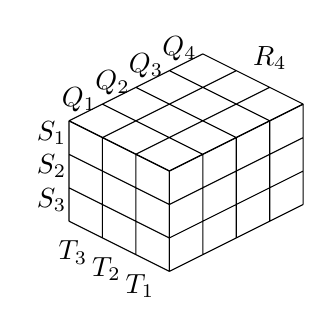
\begin{tikzpicture}[scale=0.425]

    
  \draw[yslant=-0.5] (1,0) grid (4,3);
  \draw[yslant=0.5] (4,-4) grid (8,-1);
  \draw[yslant=0.5,xslant=-1] (3,-1) grid (7,2);
\node[anchor=south west] at (-0.25,1.5,0) {$S_1$};
\node[anchor=south west] at (-0.25,0.5,0) {$S_2$};
\node[anchor=south west] at (-0.25,-0.5,0) {$S_3$};
\node[anchor=north west] at (0.5,3.8,0) {$Q_1$};
\node[anchor=north west] at (1.5,4.3,0) {$Q_2$};
\node[anchor=north west] at (2.5,4.8,0) {$Q_3$};
\node[anchor=north west] at (3.5,5.3,0) {$Q_4$};
\node[anchor=north west] at (0.4,-0.8,0) {$T_3$};
\node[anchor=north west] at (1.4,-1.3,0) {$T_2$};
\node[anchor=north west] at (2.4,-1.8,0) {$T_1$};
\node[anchor=north] at (7,5,0) {$R_4$};
\end{tikzpicture}}\\
\end{tabular}
    
\end{center}

\caption{The third candidate allocation $A''=(S_1',Q_2^*)$. We use blue for bundle $S_1'  \subseteq S_1$ and green color for $Q_2^*\subseteq Q_2$. The cut $C=\{T_2^* \cup Q_1^*\}$ is shown with a thick line. Note that the allocation is valid and none of the bundles intersects with $R_4$. We try to apply Corollary \ref{cor:2agents} for agents $T$ and $R$ and the set of items $M \setminus (T_2^*\cup Q_1^*)$. We could construct a similar allocation for any bundle $S_i'$ and bundle $Q_j$ by renaming the bundles such that $S_i' \cap Q_j^* = \emptyset$ and $S_i' \cap R_4 = \emptyset$.}
\label{fig:4agents3}
\end{figure}


   Otherwise, it should be that for the cut $C=S'_1\cup Q^*_2$ there exist two sets $T_1',T_2' \in \mathcal{X}_{T}(C)$. 
    Since for any $j \in \{1,2\}$, $T_j'\subseteq S'_1\cup Q^*_2$, by \eqref{eq:4agentsCond2} and \eqref{eq:4agentsCond3} it holds that 
      \begin{equation}
        \label{eq:4agentsCond4}
        T_j' \cap Q^*_3 = \emptyset, T_j' \cap S'_2 = \emptyset \mbox{ and } T_j' \cap R_4 = \emptyset, \mbox{ for } j \in \{1,2\}\,.
    \end{equation}
    



\begin{figure}[t]
\begin{center}

    \begin{tabular}{cc}
\small{
\begin{tikzpicture}[scale=0.425]
\draw[yslant=0.5,ultra thick, black] (5,-4) rectangle +(1,3);
\draw[yslant=0.5,ultra thick, black](4,-2) rectangle +(1,1); \draw[yslant=0.5,xslant=-1,ultra thick, black](5,1) rectangle +(-2,-2);   

\draw[yslant=0.5,xslant=-1,ultra thick, black](7,1) rectangle +(-2,-1); 
\draw[yslant=-0.5,ultra thick, black](4,3) rectangle +(-2,-1);

\draw[yslant=0.5,xslant=-1,ultra thick, white](5,1) rectangle +(0,-1); 

\draw[yslant=0.5,ultra thick, white] (5,-2) rectangle +(0,1);


\draw[yslant=0.5,pattern={crosshatch dots},pattern color=green] (6,-4) rectangle +(1,3);
\draw[yslant=0.5,pattern={north west lines},pattern color=red] (5,-4) rectangle +(1,3);
\draw[yslant=0.5,pattern={north west lines},pattern color=red] (4,-2) rectangle +(2,1);
\draw[yslant=0.5,xslant=-1,pattern={crosshatch dots},pattern color=green](6,0) rectangle +(-1,-1); 
\draw[yslant=0.5,pattern={horizontal lines},pattern color=blue](4,-3) rectangle +(1,1);    
%\draw[yslant=0.5,xslant=-1,pattern={north west lines},pattern color=red](7,1) rectangle +(-4,-1);
\draw[yslant=0.5,xslant=-1,pattern={north west lines},pattern color=red](5,0) rectangle +(-2,-1);
\draw[yslant=-0.5,pattern={horizontal lines},pattern color=blue](4,2) rectangle +(-3,-1);     
\draw[yslant=-0.5,pattern={north west lines},pattern color=red](4,3) rectangle +(-1,-1);    
  \draw[yslant=-0.5] (1,0) grid (4,3);
  \draw[yslant=0.5] (4,-4) grid (8,-1);
  \draw[yslant=0.5,xslant=-1] (3,-1) grid (7,2);
\node[anchor=south west] at (-0.25,1.5,0) {$S_1$};
\node[anchor=south west] at (-0.25,0.5,0) {$S_2$};
\node[anchor=south west] at (-0.25,-0.5,0) {$S_3$};
\node[anchor=north west] at (0.5,3.8,0) {$Q_1$};
\node[anchor=north west] at (1.5,4.3,0) {$Q_2$};
\node[anchor=north west] at (2.5,4.8,0) {$Q_3$};
\node[anchor=north west] at (3.5,5.3,0) {$Q_4$};
\node[anchor=north west] at (0.4,-0.8,0) {$T_3$};
\node[anchor=north west] at (1.4,-1.3,0) {$T_2$};
\node[anchor=north west] at (2.4,-1.8,0) {$T_1$};
\node[anchor=north] at (7,5,0) {$R_1$};
\end{tikzpicture}}
&
\small{
\begin{tikzpicture}[scale=0.425]
\draw[yslant=0.5,ultra thick, black] (5,-4) rectangle +(1,3);
\draw[yslant=0.5,ultra thick, black](4,-2) rectangle +(1,1); \draw[yslant=0.5,xslant=-1,ultra thick, black](5,1) rectangle +(-2,-2);   

\draw[yslant=0.5,xslant=-1,ultra thick, black](7,1) rectangle +(-2,-1); 
\draw[yslant=-0.5,ultra thick, black](4,3) rectangle +(-2,-1);

\draw[yslant=0.5,xslant=-1,ultra thick, white](5,1) rectangle +(0,-1); 

\draw[yslant=0.5,ultra thick, white] (5,-2) rectangle +(0,1);
\draw[yslant=0.5,pattern={crosshatch dots},pattern color=green] (6,-4) rectangle +(1,3);
\draw[yslant=0.5,pattern={north west lines},pattern color=red] (5,-4) rectangle +(1,3);
\draw[yslant=0.5,pattern={north west lines},pattern color=red] (4,-2) rectangle +(2,1);
\draw[yslant=0.5,xslant=-1,pattern={crosshatch dots},pattern color=green](6,0) rectangle +(-1,-1); 
\draw[yslant=0.5,pattern={horizontal lines},pattern color=blue](4,-3) rectangle +(1,1);    
%\draw[yslant=0.5,xslant=-1,pattern={north west lines},pattern color=red](7,1) rectangle +(-4,-1);
\draw[yslant=0.5,xslant=-1,pattern={north west lines},pattern color=red](5,0) rectangle +(-2,-1);
\draw[yslant=-0.5,pattern={horizontal lines},pattern color=blue](4,2) rectangle +(-3,-1);     
\draw[yslant=-0.5,pattern={north west lines},pattern color=red](4,3) rectangle +(-1,-1);    
  \draw[yslant=-0.5] (1,0) grid (4,3);
  \draw[yslant=0.5] (4,-4) grid (8,-1);
  \draw[yslant=0.5,xslant=-1] (3,-1) grid (7,2);
\node[anchor=south west] at (-0.25,1.5,0) {$S_1$};
\node[anchor=south west] at (-0.25,0.5,0) {$S_2$};
\node[anchor=south west] at (-0.25,-0.5,0) {$S_3$};
\node[anchor=north west] at (0.5,3.8,0) {$Q_1$};
\node[anchor=north west] at (1.5,4.3,0) {$Q_2$};
\node[anchor=north west] at (2.5,4.8,0) {$Q_3$};
\node[anchor=north west] at (3.5,5.3,0) {$Q_4$};
\node[anchor=north west] at (0.4,-0.8,0) {$T_3$};
\node[anchor=north west] at (1.4,-1.3,0) {$T_2$};
\node[anchor=north west] at (2.4,-1.8,0) {$T_1$};
\node[anchor=north] at (7,5,0) {$R_2$};
\end{tikzpicture}}\\
\small{
\begin{tikzpicture}[scale=0.425]
\draw[yslant=0.5,ultra thick, black] (5,-4) rectangle +(1,3);
\draw[yslant=0.5,ultra thick, black](4,-2) rectangle +(1,1); \draw[yslant=0.5,xslant=-1,ultra thick, black](5,1) rectangle +(-2,-2);   

\draw[yslant=0.5,xslant=-1,ultra thick, black](7,1) rectangle +(-2,-1); 
\draw[yslant=-0.5,ultra thick, black](4,3) rectangle +(-2,-1);

\draw[yslant=0.5,xslant=-1,ultra thick, white](5,1) rectangle +(0,-1); 

\draw[yslant=0.5,ultra thick, white] (5,-2) rectangle +(0,1);
\draw[yslant=0.5,pattern={crosshatch dots},pattern color=green] (6,-4) rectangle +(1,3);
\draw[yslant=0.5,pattern={north west lines},pattern color=red] (5,-4) rectangle +(1,3);
\draw[yslant=0.5,pattern={north west lines},pattern color=red] (4,-2) rectangle +(2,1);
\draw[yslant=0.5,xslant=-1,pattern={crosshatch dots},pattern color=green](6,0) rectangle +(-1,-1); 
\draw[yslant=0.5,pattern={horizontal lines},pattern color=blue](4,-3) rectangle +(1,1);    
%\draw[yslant=0.5,xslant=-1,pattern={north west lines},pattern color=red](7,1) rectangle +(-4,-1);
\draw[yslant=0.5,xslant=-1,pattern={north west lines},pattern color=red](5,0) rectangle +(-2,-1);
\draw[yslant=-0.5,pattern={horizontal lines},pattern color=blue](4,2) rectangle +(-2,-1);     
\draw[yslant=-0.5,pattern={north west lines},pattern color=red](4,3) rectangle +(-1,-1);    
  \draw[yslant=-0.5] (1,0) grid (4,3);
  \draw[yslant=0.5] (4,-4) grid (8,-1);
  \draw[yslant=0.5,xslant=-1] (3,-1) grid (7,2);
\node[anchor=south west] at (-0.25,1.5,0) {$S_1$};
\node[anchor=south west] at (-0.25,0.5,0) {$S_2$};
\node[anchor=south west] at (-0.25,-0.5,0) {$S_3$};
\node[anchor=north west] at (0.5,3.8,0) {$Q_1$};
\node[anchor=north west] at (1.5,4.3,0) {$Q_2$};
\node[anchor=north west] at (2.5,4.8,0) {$Q_3$};
\node[anchor=north west] at (3.5,5.3,0) {$Q_4$};
\node[anchor=north west] at (0.4,-0.8,0) {$T_3$};
\node[anchor=north west] at (1.4,-1.3,0) {$T_2$};
\node[anchor=north west] at (2.4,-1.8,0) {$T_1$};
\node[anchor=north] at (7,5,0) {$R_3$};
\end{tikzpicture}}
&

\small{
\begin{tikzpicture}[scale=0.425]
\draw[yslant=0.5,pattern={vertical lines},pattern color=magenta] (4,-4) rectangle +(4,3);
\draw[yslant=-0.5,pattern={vertical lines},pattern color=magenta](4,3) rectangle +(-3,-3);
\draw[yslant=0.5,xslant=-1,pattern={vertical lines},pattern color=magenta] (7,2) rectangle +(-4,-3);
    
  \draw[yslant=-0.5] (1,0) grid (4,3);
  \draw[yslant=0.5] (4,-4) grid (8,-1);
  \draw[yslant=0.5,xslant=-1] (3,-1) grid (7,2);
\node[anchor=south west] at (-0.25,1.5,0) {$S_1$};
\node[anchor=south west] at (-0.25,0.5,0) {$S_2$};
\node[anchor=south west] at (-0.25,-0.5,0) {$S_3$};
\node[anchor=north west] at (0.5,3.8,0) {$Q_1$};
\node[anchor=north west] at (1.5,4.3,0) {$Q_2$};
\node[anchor=north west] at (2.5,4.8,0) {$Q_3$};
\node[anchor=north west] at (3.5,5.3,0) {$Q_4$};
\node[anchor=north west] at (0.4,-0.8,0) {$T_3$};
\node[anchor=north west] at (1.4,-1.3,0) {$T_2$};
\node[anchor=north west] at (2.4,-1.8,0) {$T_1$};
\node[anchor=north] at (7,5,0) {$R_4$};
\end{tikzpicture}}\\
\end{tabular}
    
\end{center}
\caption{The final allocation $A^*=(S_2',T_1',Q_3^*,R_4)$. We use blue for bundle $S_2' \subseteq S_2$, red for bundle $T_1' \subseteq T_1$, and green for $Q_3^* \subseteq Q_3$. We use magenta to denote bundle $R_4$. The cut is shown with a thick line $C=\{S_1',Q_3^*\}$ The allocation is valid.}
\label{fig:4agents4}
\end{figure}



    {\bf Final allocation.} Finally, we offer the allocation $A^*=(S_2',T_1',Q_3^*,R_4)$ which is valid and each agent has value at least $1/2$ for their allocated bundle. Hence, the lemma follows. Figure \ref{fig:4agents4} illustrates the allocation.
\end{proof}






As a corollary of Lemma~\ref{Lemma:4agents}, a 1/2-MMS allocation always
exists for four agents (by Observation 1); this bound is also
tight \cite{GhodsiHSSY22}. 
\begin{corollary}
\label{cor:4agents}
    A $1/2$-MMS allocation exists for four agents with subadditive valuation functions. 
\end{corollary}

\subsection{Many agents}
\label{sec:MoreAgents}
In this section, we demonstrate how our arguments developed in the previous sections can be useful towards proving positive results for the case of multiple agents. Indeed, we show the existence of $1/2$-MMS allocations for multiple agents, when they have one of two admissible valuation functions.

\begin{theorem}\label{thm:two-types}
    For every instance of $n$ agents, where each agent $i$ has a valuation function  $v_i \in \{v_S,v_T\}$, for any subadditive valuation functions $v_S,v_T$, there exists a $1/2$-MMS allocation.
\end{theorem}
\begin{proof}

   
    The proof is by induction on the number of agents. At the induction step we guarantee that $\mu_i$ for each remaining agent $i$ does not decrease, so at the end they will receive at least $1/2$ of their original $\mu_i$ value. For $n=2$ the theorem follows by Corollary \ref{cor:2agents}. 
    Let's assume that the statement holds for less than $n$, we will show that it also works for $n$ agents. Let $n_S$ and $n_T$ be the number of agents with valuation function $v_S$ (agents of type $S$), and $v_T$ (agents of type $T$). Note that $n_S + n_T = n$.  W. l. o. g. assume that $n_S\ge n_T$ and hence $n_S \ge \left\lceil \frac{n}{2}\right\rceil$ and $n_T \le \left\lfloor \frac{n}{2}\right\rfloor$. Let also $S_j$ and $T_j$ be the $j$-th MMS bundle of an agent of type $S$ and $T$, respectively.
    
    We consider the cut $C=\bigcup_{j=1}^{\lfloor n/2\rfloor}T_j$, i.e., the union of the first $\lfloor n/2\rfloor$ MMS bundles of the agents of type $T$; note that both $C$ and $M\setminus C$ contain at least $\lfloor n/2\rfloor$ such MMS bundles.
    Then, we consider the maximum desired half, $\mathcal{X}_{S}^{*}(C)$, of agents of type $S$ over $C$. 
    Let $n'=\min\{\lvert \mathcal{X}_{S}^{*}(C) \rvert,n_S\}$, and by Observation~\ref{obs:Cut_noOfDesiredSets}, $n' \ge \left\lceil\frac{n}{2}\right\rceil$. This implies that there exist $n'$ mutually disjoint bundles, each of which has value at least $1/2$ for the agents of type $S$. Suppose that we assign those bundles to $n'\leq n_S$ agents of type $S$. 
    
    Let $M'$ be the union of those bundles, then it holds that $M'$ is disjoint with either $C$ or $M\setminus C$,  therefore $M'$ is disjoint with at least $\lfloor n/2\rfloor \geq n-n'$ MMS bundles of agents of type $T$. Moreover $M'$ is a subset of $n'$ MMS bundles of agents of type $S$, therefore $M'$ is disjoint with $n-n'$ MMS bundles of agents of type $S$. Altogether,  we are left with a reduced instance with $n-n'$ agents, where each remaining agent $i$  can partition the remaining items $M\setminus M'$ into at least $n-n'$ bundles of value at least $\mu_i^n(M)$, since $\mu_i^{n-n'}(M\setminus M')\geq \mu_i^n(M)$.  By the induction hypothesis there exists a $1/2$-MMS allocation for the reduced instance, and by combining it with the allocation of $M'$ to the $n'$ agents the proof is complete.
\end{proof}

 \section{$\boldsymbol{\alpha}$-MMS($\mathbf{d}$) for subadditive valuations}
\label{sec:Reductions}
In this section, we present a thorough study of conditions of existence (and non-existence) of $\boldsymbol{\alpha}$-MMS($\mathbf{d}$) allocations for various combinations of $\boldsymbol{\alpha}$ and $\mathbf{d}$. We provide two characterization results for three agents and several impossibility results for many agents. 

\subsection{Three Agents}
 In this section we consider three agents with subadditive valuations, and we fully characterize the conditions of existence of $1/2$-MMS$(\mathbf{d})$  (Theorem~\ref{thm:three-general}) and of $(1,1/2,1/2)$-MMS$(\mathbf{d})$ allocations (Theorem~\ref{thm:three-general-approximate}), with respect to any vector $\mathbf{d}$. We prove those results via a series of Lemmas and Corollaries in Sections~\ref{sec:CharacterizationLemmas}~and~\ref{sec:ManyAgentsImpossib}.

 We give a key claim (Claim~\ref{cl:disjointAllocations}) to be used as a technical tool in the follow up lemmas; if there exist two allocations that ``satisfy'' all but one agent, and those allocations are disjoint in one MMS bundle of the last agent, then one of the two allocations will leave items that the last agent values by at least $1/2$. Hence, that allocation can be extended to include the last agent that is guaranteed to receive at least $1/2$. 

 \begin{claim}
\label{cl:disjointAllocations}
    Consider any instance of $n$ agents, and any vectors ${\bf d}=(d_1,\ldots, d_n)$ and $\boldsymbol{\alpha}=(\alpha_1,\ldots,\alpha_n)$ with $\alpha_n =1/2$. If there exist two  allocations $A$ and $A'$, that are both $\boldsymbol{\alpha}_{-n}$-MMS$({\bf d}_{-n})$ for the first $n-1$ agents, such that there exists an MMS bundle $X$ of the last agent, where $X \cap \left(\bigcup_{Y\in A}Y\right)$ and $X \cap \left(\bigcup_{Y'\in A'}Y'\right)$ are disjoint,  
    then there exists a $\boldsymbol{\alpha}$-MMS$(\bf d)$ allocation for all $n$ agents.
\end{claim}


    
\begin{proof}
    The last agent values by at least $1/2$ either $X\cap \left(\bigcup_{Y\in A}Y\right)$ or $X\setminus \left(\bigcup_{Y\in A}Y\right) \subseteq X\cap \left(\bigcup_{Y'\in A'}Y'\right)$. W.l.o.g. suppose that the former holds. Then, the allocation where the last agent gets $X\cap \left(\bigcup_{Y\in A}Y\right) $ and the others get their allocated bundle in $A'$ is valid and it is $\boldsymbol{\alpha}$-MMS$(\bf d)$.
\end{proof}
 



\subsubsection{Characterizations of $1/2$-MMS($\mathbf{d}$) guarantees}
In this section we provide a complete characterization of results regarding $1/2$-MMS$(\mathbf{d})$ for three agents with subadditive valuations, for any vector $\mathbf{d}=(d_1,d_2,d_3)$. We summarize the results in the following theorem; note that we use the value $\sum_{i=1}^3d_i$ to distinguish among different $\mathbf{d}$, however, we do not claim that there is any strong correlation. 

\begin{theorem}\label{thm:three-general}
    A $1/2$-MMS$(\mathbf{d})$ allocation exists for three agents with subadditive valuation functions, when (i) $\mathbf{d}=(3,2,2)$ or (ii)  $\sum_{i=1}^3(d_i)\geq 8$ and $d_i=1$ for at most one agent $i$. In any other case, there exists an instance with no $1/2$-MMS$(\mathbf{d})$ allocation.
\end{theorem}
\begin{proof}
    The positive results are derived by using Observation~\ref{obs:simpleReduction} and showing that there is always a $1/2$-MMS$(3,2,2)$ allocation (Lemma~\ref{Lemma:threehalfs}), and a $(1,1/2,1/2)$-MMS$(\mathbf{d})$ allocation, for $\mathbf{d}=(5,2,1)$ (Lemma~\ref{lem:(5,2,1)}), $\mathbf{d}=(4,3,1)$ (Lemma~\ref{lem:(4,3,1)}), and $\mathbf{d}=(4,2,2)$  (Lemma~\ref{lemma:3Agents4}). 
    
    The impossibility results are derived by using Observation~\ref{obs:simpleReduction} and showing that for any of the following $\mathbf{d}$, there exists an instance that no $1/2$-MMS$(\mathbf{d})$ allocation exists. This is shown for $\mathbf{d}=(k,1,1)$, for any $k\geq 1$ (Corollary~\ref{cor:d_i<k}), $\mathbf{d}=(4,2,1)$ (Lemma~\ref{lem:imposs(4,2,1)}), $\mathbf{d}=(3,3,1)$ (Lemma~\ref{lem:imposs(3,3,1)}), and $\mathbf{d}=(2,2,2)$ (Lemma~\ref{lem:nagentsImp1}). 
    
    All Lemmas and Corollaries appear in Sections \ref{sec:CharacterizationLemmas}~and~\ref{sec:ManyAgentsImpossib}.
\end{proof}





\subsubsection{Characterizations of $(1,1/2,1/2)$-MMS$(\bf d)$ guarantees }
In this section we provide a complete characterization of results regarding $(1,1/2,1/2)$-MMS$(\bf d)$ for three agents with subadditive valuations.

\begin{theorem}\label{thm:three-general-approximate}
    A $(1,1/2,1/2)$-MMS$(\bf d)$ allocation exists for three agents with subadditive valuation functions, when $\sum_{i=1}^3(d_i)\geq 8$, when $d_i=1$ for at most one agent $i$, and $\max_i d_i \geq 4$. In any other case, there exists an instance with no $1/2$-MMS$(\mathbf{d})$ allocation.
\end{theorem}

\begin{proof}
    The positive results are derived by using Observation~\ref{obs:simpleReduction} and showing that there is always a  $(1,1/2,1/2)$-MMS$(\mathbf{d})$ allocation, for $\mathbf{d}=(5,2,1)$ (Lemma~\ref{lem:(5,2,1)}), $\mathbf{d}=(4,3,1)$ (Lemma~\ref{lem:(4,3,1)}) and $\mathbf{d}=(4,2,2)$ (Lemma~\ref{lemma:3Agents4}). 
    
    The impossibility results are derived by using Observation~\ref{obs:simpleReduction} and showing that for any of the following $\mathbf{d}$, there exists an instance that no $1/2$-MMS$(\mathbf{d})$ allocation exists. This is shown for $\mathbf{d}=(k,1,1)$, for any $k\geq 1$ (Corollary~\ref{cor:d_i<k}), $\mathbf{d}=(4,2,1)$ (Lemma~\ref{lem:imposs(4,2,1)}), and $\mathbf{d}=(3,3,3)$ (Lemma~\ref{lem:imposs(3,3,3)}).

    All Lemmas and Corollaries appear in Sections \ref{sec:CharacterizationLemmas}~and~\ref{sec:ManyAgentsImpossib}.
    \end{proof}

\subsubsection{$\alpha$-MMS$(\bf d)$ guarantees for three agents}
\label{sec:CharacterizationLemmas}

In this section we give a series of lemmas regarding the existence of $1/2$-MMS$(\bf d)$ and $(1,1/2,1/2)$-MMS$(\bf d)$ allocations, or their impossibilities, for three agents. Those lemmas are used in the characterizations of the existence of $1/2$-MMS$(\bf d)$ and $(1,1/2,1/2)$-MMS$(\bf d)$ allocations of the previous sections, focusing on results for three agents.


    \begin{lemma}
\label{lem:imposs(4,2,1)}
There exists an instance of three agents with subadditive valuation functions, where no $1/2$-MMS$(4,2,1)$ allocation exists.
\end{lemma}

\begin{proof}
    Consider an instance with $M=\{h,g_1,g_2,g_3\}$, where $v_1(S)=1$ for any $S\subseteq M$, $v_2(S)=1$, if $h\in S$, otherwise $v_2(S)=1/3 \cdot |S|$, and the last agent has an additive valuation function over $M$, with $v_3(h)=1/3$ and $v_3(g)=2/9$ for any $g\neq h$. Note that the first agent can partition $M$ into four bundles, each valued at $1$, the second agent can partition $M$ into $(\{h\},\{g_1,g_2,g_3\})$, valuing each bundle at $1$, and the third agent values $M$ at $1$.

    Suppose that there exists an allocation $A$ that is $1/2$-MMS$(4,2,1)$. If $h\in A_3$, then the third agent should receive at least one more item. Then, the second agent should receive two items other than $h$ to form a bundle with a value of at least $1/2$ to her; this leaves no items for the first agent. If $h\notin A_3$, the third agent must receive all remaining items to form a bundle with a value of at least $1/2$. This leaves one item for each of the first two agents. We conclude that no such allocation $A$ exists.  
\end{proof}

\begin{lemma} 
\label{lem:(5,2,1)}
A $(1,1/2,1/2)$-MMS$(5,2,1)$ allocation exists for three agents with subadditive valuation functions.
\end{lemma}
\begin{proof}
    We denote by $S,T,Q$ the three agents, and by $S_j,T_j,Q_j$ their $j$-th MMS bundle, respectively. 
    Consider all the cuts $C_{ijk}=\{S_i \cup S_j \cup S_k\}$ that we offer to $T$. We first show the following claim:
    \begin{claim}
        There exists a cut $C_{ijk}$, such that $v_T(T_1\cap C_{ijk})\geq 1/2$ and $v_T(T_2\cap C_{ijk})\geq 1/2$. 
    \end{claim}
    \begin{proof}
        Suppose on the contrary that there is no such cut. Then, for each $C_{ijk}$, agent $T$ has value at least $1/2$ for the intersection of $C_{ijk}$ and either $T_1$ or $T_2$ (but not both due to our assumption). The reason is that if $T$'s value was less than $1/2$ for both intersections, due to subadditivity any $C_{i'j'k'}$ for which $C_{ijk} \cup C_{i'j'k'}=M$ would contradict our assumption. 
        Let $\phi(C_{ijk})=1$ if $T$ has value at least $1/2$ for the intersection with $T_1$, otherwise, $\phi(C_{ijk})=2$.

        W.l.o.g. suppose that  $\phi(C_{123})=1$, then $\phi(C_{145})=2$, o.w. $v_T(C_{123}\cap T_2)+v_2(C_{145}\cap T_2)<1$, which is a contradiction to subadditivity, since the union of those two sets is $T_2$, and $v(T_2)\geq 1$. Similarly $\phi(C_{245})=2$ and $\phi(C_{345})=2$. 
        For the same reason, since $\phi(C_{145})=2$, it should be that $\phi(C_{234})=1$, and then $\phi(C_{125})=2$. Finally it should be $\phi(C_{345})=1$, but we argue above that $\phi(C_{345})=2$, which is a contradiction to our assumption. 
    \end{proof}  


        
    W.l.o.g. suppose that $C_{123}$ is the cut satisfying the statement of the above claim. Then, $T$ has value at least $1/2$ for both $T_1^*=T_1\cap C_{123}$ and $T_2^*=T_2\cap C_{123}$ (Figure \ref{fig:3agents521}(a)). Then, the allocations $A=(S_4,T_1^*)$ and  $A'=(S_5,T_2^*)$ for agents $S$ and $T$ are $(1,1/2)$-MMS$(5,2)$ and they are disjoint (Figures \ref{fig:3agents521}(b) and \ref{fig:3agents521}(c) resp.). By Claim~\ref{cl:disjointAllocations} the lemma follows. 
\end{proof}


\begin{center}
\begin{figure}[t] 
\begin{center}
    \begin{tabular}{ccc}
\begin{tikzpicture}[scale=0.45]
\draw[black, ultra thick](0,2) rectangle +(2,3);
\draw[pattern={north west lines},pattern color=red]
(0,2) rectangle +(2,3);
  \draw[step=1cm,] (0,0) grid (2,5);

\node[anchor=north] at (0.5,6.25) {$T_1$};
\node[anchor=north] at (1.5,6.25) {$T_2$};
\node[anchor=west] at (-1.5,0.5) {$S_5$};
\node[anchor=west] at (-1.5,1.5) {$S_4$};
\node[anchor=west] at (-1.5,2.5) {$S_3$};
\node[anchor=west] at (-1.5,3.5) {$S_2$};
\node[anchor=west] at (-1.5,4.5) {$S_1$};
\end{tikzpicture} & \begin{tikzpicture}[scale=0.45]
%\draw[black, ultra thick](0,2) rectangle +(2,3);
\draw[pattern={north west lines},pattern color=red]
(0,2) rectangle +(1,3);
\draw[pattern={horizontal lines},pattern color=blue](0,1) rectangle +(2,1);
  \draw[step=1cm,] (0,0) grid (2,5);

\node[anchor=north] at (0.5,6.25) {$T_1$};
\node[anchor=north] at (1.5,6.25) {$T_2$};
\node[anchor=west] at (-1.5,0.5) {$S_5$};
\node[anchor=west] at (-1.5,1.5) {$S_4$};
\node[anchor=west] at (-1.5,2.5) {$S_3$};
\node[anchor=west] at (-1.5,3.5) {$S_2$};
\node[anchor=west] at (-1.5,4.5) {$S_1$};
\end{tikzpicture} &
\begin{tikzpicture}[scale=0.45]
%\draw[black, ultra thick](0,2) rectangle +(2,3);
\draw[pattern={north west lines},pattern color=red]
(1,2) rectangle +(1,3);
\draw[pattern={horizontal lines},pattern color=blue](0,0) rectangle +(2,1);
  \draw[step=1cm,] (0,0) grid (2,5);

\node[anchor=north] at (0.5,6.25) {$T_1$};
\node[anchor=north] at (1.5,6.25) {$T_2$};
\node[anchor=west] at (-1.5,0.5) {$S_5$};
\node[anchor=west] at (-1.5,1.5) {$S_4$};
\node[anchor=west] at (-1.5,2.5) {$S_3$};
\node[anchor=west] at (-1.5,3.5) {$S_2$};
\node[anchor=west] at (-1.5,4.5) {$S_1$};
\end{tikzpicture}\\
(a) & (b) & (c) \\
    \end{tabular}
    \end{center}
\caption{In (a), with a thick line we show the cut $C=C_{123}$, and the red bundles correspond to $T_1^*,T_2^*$. In (b) and (c), we illustrate the allocations $A$ and $A'$, respectively; agent $S$ gets a whole bundle in each allocation (denoted with blue color).}
\label{fig:3agents521}
\end{figure}  
\end{center}



\begin{lemma} 
\label{lem:(4,3,1)}
A $(1,1/2,1/2)$-MMS$(4,3,1)$ allocation exists for three agents with subadditive valuation functions.  
\end{lemma}
\begin{center}
\begin{figure} 
\begin{center}
    \begin{tabular}{ccc}
\begin{tikzpicture}[scale=0.45]
%(0,0) rectangle +(1,2);
%\draw[pattern={north west lines},pattern color=red]
(0,0) rectangle +(1,2);
\draw[black, ultra thick](0,2) rectangle +(3,2);
\draw[pattern={north west lines},pattern color=red]
(0,2) rectangle +(2,2);
  \draw[step=1cm,] (0,0) grid (3,4);

\node[anchor=north] at (0.5,5.25) {$T_1$};
\node[anchor=north] at (1.5,5.25) {$T_2$};
\node[anchor=north] at (2.5,5.25) {$T_3$};
\node[anchor=west] at (-1.5,0.5) {$S_4$};
\node[anchor=west] at (-1.5,1.5) {$S_3$};
\node[anchor=west] at (-1.5,2.5) {$S_2$};
\node[anchor=west] at (-1.5,3.5) {$S_1$};
\end{tikzpicture} & \begin{tikzpicture}[scale=0.45]
%(0,0) rectangle +(1,2);
\draw[pattern={north west lines},pattern color=red]
(0,2) rectangle +(1,2);
\draw[pattern={horizontal lines},pattern color=blue](0,1) rectangle +(3,1);
  \draw[step=1cm,] (0,0) grid (3,4);

\node[anchor=north] at (0.5,5.25) {$T_1$};
\node[anchor=north] at (1.5,5.25) {$T_2$};
\node[anchor=north] at (2.5,5.25) {$T_3$};
\node[anchor=west] at (-1.5,0.5) {$S_4$};
\node[anchor=west] at (-1.5,1.5) {$S_3$};
\node[anchor=west] at (-1.5,2.5) {$S_2$};
\node[anchor=west] at (-1.5,3.5) {$S_1$};
\end{tikzpicture} &
\begin{tikzpicture}[scale=0.45]
\draw[pattern={north west lines},pattern color=red]
(1,2) rectangle +(1,2);
\draw[pattern={horizontal lines},pattern color=blue](0,0) rectangle +(3,1);
  \draw[step=1cm,] (0,0) grid (3,4);

\node[anchor=north] at (0.5,5.25) {$T_1$};
\node[anchor=north] at (1.5,5.25) {$T_2$};
\node[anchor=north] at (2.5,5.25) {$T_3$};
\node[anchor=west] at (-1.5,0.5) {$S_4$};
\node[anchor=west] at (-1.5,1.5) {$S_3$};
\node[anchor=west] at (-1.5,2.5) {$S_2$};
\node[anchor=west] at (-1.5,3.5) {$S_1$};
\end{tikzpicture}\\
(a) & (b) & (c) \\
    \end{tabular}
    \end{center}
\caption{In (a), with a thick line we show the cut $C=\{S_1 \cup S_2\}$. Red bundles correspond to $T_1^*,T_2^*$ (a). In (b) and (c), we illustrate allocations $A$ and $A'$, respectively; agent $S$ gets a whole bundle in each allocation (denoted with blue color).}
\label{fig:3agents431}
\end{figure}  
\end{center}

\begin{proof}
    We denote by $S,T,Q$ the three agents, and by $S_j,T_j,Q_j$ their $j$-th MMS bundle, respectively. Consider the cut $C={S_1\cup S_2}$ that we offer to $T$. W.l.o.g., suppose that
    $\mathcal{X}^*_T(C)=\mathcal{X}_T(C)$ and let $T_1^*,T_2^* \in \mathcal{X}^*_T(C)$ (Figure \ref{fig:3agents431} (a)). 
    Then, the allocations $A=(S_3,T_1^*)$ and  $A'=(S_4,T_2^*)$ (Figures \ref{fig:3agents431} (b) and \ref{fig:3agents431}(c) resp.) for agents $S$ and $T$ are $(1,1/2)$-MMS$(4,3)$ and they are disjoint. By Claim~\ref{cl:disjointAllocations} the lemma follows.
\end{proof}

\begin{lemma} \label{lemma:3Agents4}
A $(1,1/2,1/2)$-MMS$(4,2,2)$ allocation exists for three agents with subadditive valuation functions. 
\end{lemma}
\begin{proof}
We denote by $S,T,Q$ the three agents, and by $S_j,T_j,Q_j$ their $j$-th MMS bundle, respectively. We show the existence of two allocations for agents $T$ and $S$ that are disjoint on some $Q_j$,   and by Claim \ref{cl:disjointAllocations} the proof completes. 

We define the cuts $C_{ij}=\{S_i \cup S_j\}$ that we offer to $T$. W.l.o.g. assume that $v_T(T'_1)\geq 1/2$, for $T_1' =T_1\cap  C_{12}$ and $v_T(T_1'')\geq 1/2$ for $T_1''=T_1 \cap C_{23}$; if this is not the case we can rename the bundles of agent $S$.  Figures \ref{fig:3agents422}(a) and \ref{fig:3agents422}(b) illustrate the bundles and the cuts, respectively. 


Next we offer the cut $C=\{(Q_1 \setminus S_1) \cup S_3\}$ to $T$ (Figure \ref{fig:3agents422a}(a)). We consider the intersection of $T_2$ with $C$, and let $T_2^*=\max\{T_2\cap C, T_2\cap (M\setminus C)\}$. Note that $M\setminus C = (Q_2 \setminus S_3) \cup S_1$, so the cut provides some symmetry between $S_1$ and $S_3$; $S_1$ intersect with $T'_1$ but not $T''_1$, and for $S_3$ is the other way around. So, no matter which set is $T_2^*$, it does not intersect either $S_1$ or $S_3$, which in turns does not intersect with either $T'_1$ or $T''_1$. Therefore it is w.l.o.g. to assume that $T_2^*=T_2\cap C$ (Figure \ref{fig:3agents422a}(a)) and then, the allocations $A=(S_1,T_2^*)$ and  $A'=(S_4,T_1'')$ (Figures \ref{fig:3agents422a}(b) and \ref{fig:3agents422a}(c) resp.) for agents $S$ and $T$ are $(1,1/2)$-MMS$(4,2)$ and they are disjoint on $Q_2$. By Claim~\ref{cl:disjointAllocations} the lemma follows.
\end{proof}

\begin{center}

\begin{figure}[t]
\begin{center}

\begin{tabular}{cc}

\small{\begin{tikzpicture}[scale=0.45]
    \draw[yslant=0.5,xslant=-1,color=black,ultra thick] (6,3) rectangle +(-2,-2);    
    \draw[yslant=0.5,color=black,ultra thick] (3,-1) rectangle +(2,2);
    \draw[yslant=-0.5,color=black,ultra thick](3,4) rectangle +(-2,-2);
    \draw[yslant=0.5,xslant=-1,pattern={north west lines},pattern color=red](6,3) rectangle +(-2,-1);
    \draw[yslant=-0.5,pattern={north west lines},pattern color=red](2,4) rectangle +(-1,-2);
  \draw[yslant=-0.5] (1,0) grid (3,4);
  \draw[yslant=0.5] (3,-3) grid (5,1);
  \draw[yslant=0.5,xslant=-1] (4,1) grid (6,3);
\node[anchor=south west] at (-0.2,2.5,0) {$S_1$};
\node[anchor=south west] at (-0.2,1.5,0) {$S_2$};
\node[anchor=south west] at (-0.2,0.5,0) {$S_3$};
\node[anchor=south west] at (-0.2,-0.5,0) {$S_4$};
\node[anchor=north west] at (0.45,4.7,0) {$Q_1$};
\node[anchor=north west] at (1.5,5.3,0) {$Q_2$};
\node[anchor=north west] at (0.5,-0.8,0) {$T_1$};
\node[anchor=north west] at (1.5,-1.2,0) {$T_2$};
\end{tikzpicture}} &
\small{\begin{tikzpicture}[scale=0.45]
     %\draw[yslant=0.5,xslant=-1,color=black,ultra thick] (6,3) rectangle +(-2,-2);    
    \draw[yslant=0.5,color=black,ultra thick] (3,-2) rectangle +(2,2);
    \draw[yslant=-0.5,color=black,ultra thick](3,3) rectangle +(-2,-2);
    %\draw[yslant=0.5,xslant=-1,pattern={north west lines},pattern color=red](6,2) rectangle +(-2,-1);
    \draw[yslant=-0.5,pattern={north west lines},pattern color=red](2,3) rectangle +(-1,-2);
    
  \draw[yslant=-0.5] (1,0) grid (3,4);
  \draw[yslant=0.5] (3,-3) grid (5,1);
  \draw[yslant=0.5,xslant=-1] (4,1) grid (6,3);
\node[anchor=south west] at (-0.2,2.5,0) {$S_1$};
\node[anchor=south west] at (-0.2,1.5,0) {$S_2$};
\node[anchor=south west] at (-0.2,0.5,0) {$S_3$};
\node[anchor=south west] at (-0.2,-0.5,0) {$S_4$};
\node[anchor=north west] at (0.45,4.7,0) {$Q_1$};
\node[anchor=north west] at (1.5,5.3,0) {$Q_2$};
\node[anchor=north west] at (0.5,-0.8,0) {$T_1$};
\node[anchor=north west] at (1.5,-1.2,0) {$T_2$};
\end{tikzpicture}} \\
(a) & (b) \\
$T_1' \in \mathcal{X}_T(C_{12})$ &  $T_1'' \in \mathcal{X}_T(C_{23})$ \\
\end{tabular}
    
\end{center}
\caption{In (a) and (b), with a thick line we show the cut $C_{12}$ and $C_{23}$, respectively. Red bundles correspond to $T_1'$ in (a) and $T_1''$ in (b).}
\label{fig:3agents422}
\end{figure} 
\end{center}


\begin{center}

\begin{figure}[t]
\begin{center}

\begin{tabular}{ccc}
\small{\begin{tikzpicture}[scale=0.45]
      
    \draw[yslant=0.5,color=black,ultra thick] (3,-2) rectangle +(2,1);
    \draw[yslant=0.5,color=black,ultra thick] (3,-3) rectangle +(1,3);
    \draw[yslant=0.5,color=black,ultra thick,white] (3,-2) rectangle +(1,1);

    \draw[yslant=0.5,pattern={north west lines},pattern color=red] (3,-3) rectangle +(1,3);
    \draw[yslant=0.5,pattern={north west lines},pattern color=red] (3,-2) rectangle +(2,1);
    \draw[yslant=-0.5,pattern={north west lines},pattern color=red](3,3) rectangle +(-1,-3);
    
    \draw[yslant=-0.5,color=black,ultra thick](3,3) rectangle +(-2,-3);
  \draw[yslant=-0.5] (1,0) grid (3,4);
  \draw[yslant=0.5] (3,-3) grid (5,1);
  \draw[yslant=0.5,xslant=-1] (4,1) grid (6,3);
\node[anchor=south west] at (-0.2,2.5,0) {$S_1$};
\node[anchor=south west] at (-0.2,1.5,0) {$S_2$};
\node[anchor=south west] at (-0.2,0.5,0) {$S_3$};
\node[anchor=south west] at (-0.2,-0.5,0) {$S_4$};
\node[anchor=north west] at (0.45,4.7,0) {$Q_1$};
\node[anchor=north west] at (1.5,5.3,0) {$Q_2$};
\node[anchor=north west] at (0.5,-0.8,0) {$T_1$};
\node[anchor=north west] at (1.5,-1.2,0) {$T_2$};
\end{tikzpicture}}
 &
 \small{\begin{tikzpicture}[scale=0.45]
    
      
    

    \draw[yslant=0.5,pattern={north west lines},pattern color=red] (3,-3) rectangle +(1,3);
    \draw[yslant=0.5,pattern={north west lines},pattern color=red] (3,-2) rectangle +(2,1);
    \draw[yslant=-0.5,pattern={north west lines},pattern color=red](3,3) rectangle +(-1,-3);
    \draw[yslant=0.5,xslant=-1,pattern={horizontal lines},pattern color=blue](3,3) (6,3) rectangle +(-2,-2);  
    \draw[yslant=0.5,pattern={horizontal lines},pattern color=blue](3,0) rectangle +(2,1);     
    \draw[yslant=-0.5,pattern={horizontal lines},pattern color=blue](3,4) rectangle +(-2,-1);  
    
     \draw[yslant=-0.5] (1,0) grid (3,4);
  \draw[yslant=0.5] (3,-3) grid (5,1);
  \draw[yslant=0.5,xslant=-1] (4,1) grid (6,3);
\node[anchor=south west] at (-0.2,2.5,0) {$S_1$};
\node[anchor=south west] at (-0.2,1.5,0) {$S_2$};
\node[anchor=south west] at (-0.2,0.5,0) {$S_3$};
\node[anchor=south west] at (-0.2,-0.5,0) {$S_4$};
\node[anchor=north west] at (0.45,4.7,0) {$Q_1$};
\node[anchor=north west] at (1.5,5.3,0) {$Q_2$};
\node[anchor=north west] at (0.5,-0.8,0) {$T_1$};
\node[anchor=north west] at (1.5,-1.2,0) {$T_2$};
\end{tikzpicture}}
 &
 \small{\begin{tikzpicture}[scale=0.45]
\draw[yslant=-0.5,pattern={north west lines},pattern color=red](2,3) rectangle +(-1,-2);
\draw[yslant=0.5,pattern={horizontal lines},pattern color=blue](3,-3) rectangle +(2,1);     
\draw[yslant=-0.5,pattern={horizontal lines},pattern color=blue](3,1) rectangle +(-2,-1);  
  \draw[yslant=-0.5] (1,0) grid (3,4);
  \draw[yslant=0.5] (3,-3) grid (5,1);
  \draw[yslant=0.5,xslant=-1] (4,1) grid (6,3);
\node[anchor=south west] at (-0.2,2.5,0) {$S_1$};
\node[anchor=south west] at (-0.2,1.5,0) {$S_2$};
\node[anchor=south west] at (-0.2,0.5,0) {$S_3$};
\node[anchor=south west] at (-0.2,-0.5,0) {$S_4$};
\node[anchor=north west] at (0.45,4.7,0) {$Q_1$};
\node[anchor=north west] at (1.5,5.3,0) {$Q_2$};
\node[anchor=north west] at (0.5,-0.8,0) {$T_1$};
\node[anchor=north west] at (1.5,-1.2,0) {$T_2$};
\end{tikzpicture}}
\\
(a) & (b) & (c) \\
$T_2^* \in \mathcal{X}_T(C)$ &  $A = \{S_1,T_2^*\}$ & $A' = \{S_4,T_1''\}$  \\
\end{tabular}
    
\end{center}
\caption{For cut $C=\{(Q_1 \setminus S_1) \cup S_3\}$, let $T_2^* \in \mathcal{X}_T(C)$ (as shown in (a)). Then, the allocations $A=(S_1,T_2^*)$ (b) and  $A'=(S_4,T_1'')$ (c) are disjoint on $Q_2$. We use blue for agent $S$ and red for agent $T$'s bundles.}
\label{fig:3agents422a}
\end{figure} 
\end{center}

 






\begin{lemma} 
\label{lem:imposs(3,3,3)}
There exists an instance of three agents with subadditive valuation functions, where no $(1,1/2,1/2)$ -MMS allocation exists.
\end{lemma}

\begin{proof}
Consider an instance with items $M=\{g(i,j,k)\mid \mbox{ for } i,j,k \le 3\}$
and the following MMS bundles for the agents:
\begin{itemize}
    \item for agent $S$: $S_i=\{g(i,j,k)\mid \forall j,k\}$ for $i\in \{1,2,3\}$,
    \item for agent $T$: $T_j=\{g(i,j,k)\mid \forall i,k\}$ for $j\in \{1,2,3\}$,
    \item for agent $Q$: $Q_k=\{g(i,j,k)\mid \forall i,j\}$ for $k\in \{1,2,3\}$.
\end{itemize}
In the following, we make the convention that $i+1 = (i\mod 3) +1$, $i+2 = (i+1 \mod 3) +1$, and similarly for the other indices $j$ and $k$. 


We will construct the values of all agents symmetrically, such that for each agent $R\in \{S,Q,T\}$, her value for set $B \subseteq M$ will be $v_R(B)=\max_i\{v_R(B \cap R_i)\}$, $v_R(R_i)=1$ for any $i\in \{1,2,3\}$, and $v_R(B)\in\{1/2+\epsilon,1/2-\epsilon\}$ for $B\subset R_i$, for some $i\in\{1,2,3\}$ (where those values will be chosen appropriately so that the valuation functions are subadditive). 
Thus we only need to define the valuation functions only for $B \subset R_i$ for any $i\in \{1,2,3\}$.

For any $R\in \{S,Q,T\}$, $i\in \{1,2,3\}$, and $B \subset R_i$ with $\lvert B\rvert \notin \{4,5\}$, 
\begin{equation}
   \label{eq:422T}
       v_R(B)=\begin{cases}
      1/2 + \epsilon, & \text{if } \lvert B\rvert \geq 6\\
      1/2 - \epsilon, & \text{if } \lvert B\rvert \leq 3
      \end{cases}
   \end{equation} 

 

Consider now the bundles of the form $B^*=R_i\cap((X_j\cap Y_{k})\cup Y_{k+1})$, for any $i,j,k\in \{1,2,3\}$, where $X$ and $Y$ are the other two agents but $R$, with $X\neq Y$. Note that the above sets $B^*$ have cardinality $4$. For any $B \subset R_i$ with $\lvert B\rvert \in \{4,5\}$ we define

\begin{equation}
   \label{eq:422T}
       v_R(B)=\begin{cases}
      1/2 + \epsilon, & \text{if $\lvert B\rvert = 4$, and $B$ is some $B^*$ bundle}\\
      1/2 - \epsilon, & \text{if $\lvert B\rvert = 4$, and $B$ is different from all $B^*$ bundle} \\
      1-v_R(R_i\setminus B), & \text{if $\lvert B\rvert = 5$}
      \end{cases}
   \end{equation} 



Subadditivity is trivially guaranteed for those valuation functions. We will only show the following claim to verify that the valuations are valid monotone valuations. 

\begin{center}
\begin{figure}[t]
\begin{center}

\begin{tabular}{ccc}
\small{\begin{tikzpicture}[scale=0.475]


\draw[yslant=0.5,pattern={north west lines},pattern color=red] (4,-3) rectangle +(1,2);
\draw[yslant=0.5,pattern={north west lines},pattern color=red] (4,-3) rectangle +(3,1);
\draw[yslant=0.5,xslant=-1,pattern={north west lines},pattern color=red](3,-1) rectangle +(1,1);
\draw[yslant=-0.5,pattern={north west lines},pattern color=red](4,3) rectangle +(-1,-2);
    
\draw[yslant=0.5,pattern={horizontal lines},pattern color=blue](4,-4) rectangle +(3,1);     
\draw[yslant=-0.5,pattern={horizontal lines},pattern color=blue](4,1) rectangle +(-3,-1); 


\draw[yslant=-0.5] (1,0) grid (4,3);
\draw[yslant=0.5] (4,-4) grid (7,-1);
\draw[yslant=0.5,xslant=-1] (3,-1) grid (6,2);
\node[anchor=south west] at (-0.25,1.5,0) {$S_1$};
\node[anchor=south west] at (-0.25,0.5,0) {$S_2$};
\node[anchor=south west] at (-0.25,-0.5,0) {$S_3$};
\node[anchor=north west] at (0.3,-0.6,0) {$T_3$};
\node[anchor=north west] at (1.3,-1.1,0) {$T_2$};
\node[anchor=north west] at (2.3,-1.6,0) {$T_1$};
\node[anchor=north west] at (0.4,3.7,0) {$Q_1$};
\node[anchor=north west] at (1.4,4.2,0) {$Q_2$};
\node[anchor=north west] at (2.4,4.7,0) {$Q_3$};
\end{tikzpicture} }
 &
 \small{\begin{tikzpicture}[scale=0.45]


 \draw[yslant=0.5,xslant=-1,pattern={crosshatch dots},pattern color=green](3,-1) rectangle +(1,1);
    \draw[yslant=0.5,pattern={crosshatch dots},pattern color=green] (4,-3) rectangle +(1,2);
     \draw[yslant=-0.5,pattern={crosshatch dots},pattern color=green](4,2) rectangle +(-3,-1);  
\draw[yslant=-0.5,pattern={crosshatch dots},pattern color=green](4,3) rectangle +(-1,-1); 

\draw[yslant=0.5,pattern={horizontal lines},pattern color=blue](4,-4) rectangle +(3,1);     
\draw[yslant=-0.5,pattern={horizontal lines},pattern color=blue](4,1) rectangle +(-3,-1); 
\draw[yslant=-0.5] (1,0) grid (4,3);
\draw[yslant=0.5] (4,-4) grid (7,-1);
\draw[yslant=0.5,xslant=-1] (3,-1) grid (6,2);
\node[anchor=south west] at (-0.25,1.5,0) {$S_1$};
\node[anchor=south west] at (-0.25,0.5,0) {$S_2$};
\node[anchor=south west] at (-0.25,-0.5,0) {$S_3$};
\node[anchor=north west] at (0.3,-0.6,0) {$T_3$};
\node[anchor=north west] at (1.3,-1.1,0) {$T_2$};
\node[anchor=north west] at (2.3,-1.6,0) {$T_1$};
\node[anchor=north west] at (0.4,3.7,0) {$Q_1$};
\node[anchor=north west] at (1.4,4.2,0) {$Q_2$};
\node[anchor=north west] at (2.4,4.7,0) {$Q_3$};
\end{tikzpicture}}\\
(a) & (b)\\
\end{tabular}\end{center}\caption{The red bundle corresponds to $T_1 \cap ((Q_1 \cap S_2) \cup S_1)$ and the blue one to $S_3$, as shown in (a). Agent $Q$ values the remaining items at $1/2-\epsilon$. In (b), the green bundle corresponds to $Q_1 \cap ((T_1 \cap S_1) \cup S_2)$ and the blue one to $S_1$. Agent $T$ values the remaining items at $1/2-\epsilon$.}
\label{fig:3agents322a}
\end{figure}
\end{center}

\begin{claim}
If $S\subset R_i$ is some $B^*$ set for $R$, then $R_i\setminus S$ is not a superset of some other $B^*$ set for $R$.
\end{claim}
\begin{proof}
First note that for any $B^*=R_i\cap((X_j\cap Y_{k})\cup Y_{k+1})$, it is $R_i\setminus B^* = R_i \cap (((X_{j+1} \cup X_{j+2})\cap Y_k)\cup Y_{k+2}) $. So, it is clear that $R_i\setminus B^*$ is a superset of bundles of the form  $R_i\cap((X_{j'}\cap Y_{k'})\cup Y_{k'+2})$, which are not considered as $B^*$. So, if $S$ is some $B^*$ set for $R$, considering $R_i$, $R_i\setminus S$ cannot be a superset of some $B^*$ set for $R$.
\end{proof}




Assume for the sake of contradiction that there exists a $(1,1/2,1/2)$-MMS allocation, $A=(A_S,A_T,A_Q)$. 
Due to the definition of the valuation functions we may assume that $A_S$ is one MMS bundle for $S$, and $A_T,A_Q$ are  subsets of one MMS bundle of $T$ and $Q$, respectively. Note that the values are symmetric and we make no assumptions for agent $S$. As a result we can prove the inaproximability of $(1/2,1,1/2)$-MMS and $(1/2,1/2,1)$-MMS.


Due to the symmetric instance, suppose w.l.o.g. that $A_S=S_3$ and $A_T\subseteq T_1$. Figure~\ref{fig:3agents322a}(a) shows an example where $T$ receives a minimum possible cardinality set;  Figure~\ref{fig:3agents322a}(b) shows the case where we considered $Q$ instead of $T$, to illustrate the symmetry. We will next show that it should be that $A_T\supset T_1\cap S_2$. 

If $|A_T|\geq 6$, clearly $A_T=T_1\setminus S_3 \supset T_1\cap S_2$.
If $|A_T| = 5$, based on the definition of the valuations, it should be that $T_1\setminus A_T$ is not a $B^*$ bundle for $T$. Note that $T_1\setminus A_T $ is a superset of $ T_1\cap S_3$ and has cardinality $4$. Therefore, $T_1\setminus A_T = T_1\cap ((Q_k\cap S_1)\cup S_3)$, for some $k\in \{1,2,3\}$, otherwise (i.e., if we replace $S_1$ with $S_2$) it would be a $B^*$ set for $T$. As a result, $A_T \supset T_1\cap S_2$. If $|A_T| = 4$, then $A_T$ should be a $B^*$ set for $T$. Since $A_T\cap S_3 =\emptyset$, $A_T$ should be of the form $A_T = T_1\cap ((Q_k\cap S_1)\cup S_2)$, for some $k\in \{1,2,3\}$, which means again that  $A_T \supset T_1\cap S_2$. 

So, in any case $A_S\cup A_T \supset (T_1\cap S_2)\cup S_3$. This leaves $Q$ with some $A_Q\subseteq Q_k$, for some $k\in\{1,2,3\}$, with $|A_Q|\leq 5$. Note that $Q_k\setminus A_Q = Q_k\cap ((T_1\cap S_2)\cup S_3)$, which $Q$ values by more than $1/2$, therefore $v_Q(A_Q)<1/2$, by the valuation definition, which contradicts the assumption of the existence of a $(1,1/2,1/2)$-MMS allocation.
\end{proof}


\subsection{Many Agents}
\label{sec:ManyAgentsImpossib}
In this section we show impossibility results regarding many agents with subadditive valuations. More specifically, we show the existence of $1/2+\epsilon$ inapproximability for any vector $\boldsymbol{d}$ (Lemma ~\ref{Lemma:upperhalf}), inapproximability up to any factor $\epsilon$ when agents have less than $n$ MMS bundles (Lemma~\ref{lem:nagentsImp1}) or for MMS($n,\ldots,n,\left\lfloor\frac{n}{3}\right\rfloor$) bundles (Lemma~\ref{lem:imposs(3,3,1)}). Our last Lemma shows that any inapproximability result for $1/2$-MMS$(\mathbf{d})$ implies an inapproximability for $(1/3+\epsilon)$-MMS$(\mathbf{d})$ (Lemma~\ref{Lemma:upperBound}).

\begin{lemma}\label{Lemma:upperhalf}
    For any number of agents $n$ and any vector $\boldsymbol{d}=(d_1,\ldots, d_n)$ there exists an instance, where agents have subadditive valuations,  where no $(1/2+\epsilon)$-MMS$(\boldsymbol{d})$ allocation exists, for any $\epsilon>0$. 
\end{lemma}
\begin{proof}
    We will construct a counterexample in which every set $S \subseteq M$ has value either $1/2$ or $1$ for each agent $i$. Those valuations are carefully constructed so that if an agent receives more than $1/2$ value, it is impossible for any other agent to receive more than $1/2$.

    We consider a set of $\prod_{i=1}^n d_i$ items, that we denote as $M = \left\{g(r_1,\ldots,r_n),r_i \le d_i\right\}$.
    Let the bundle $B_{i,j}=\left\{g(r_1,\ldots,r_n):r_i=j\right\}$, for all $i\leq  n$ and $j \le d_i$. We construct the functions of each agent $i$ and set of items $S \subseteq M$ as follows:
    $$v_i\left(S\right) = \begin{cases}
        0 & \text{if } S = \emptyset\\
        1 & \text{if } \exists j: B_{i,j} \subseteq S \\
        1/2 & \text{otherwise}\\
    \end{cases}$$
Observe that the functions are subbaditive, and that for each agent $i$, $v_i(M)=1$, and there exists a partition of the items into $d_i$ bundles, namely $B_{i,1},\ldots,B_{i,d_i}$, where agent $i$ has value $1$ for each of them.

Consider any arbitrary pair of agents $i \ne i'$, then  $B_{i,j} \cap B_{i',j'} = \left\{g(r_1,\ldots,r_n):r_i=j,r_{i'}=j'\right\}$ for every pair $(j,j')$. Assume for the sake of contradiction that there exists an $(1/2+\epsilon)$-MMS$(\boldsymbol{d})$ allocation, in which bundles $A_i$ and $A_{i'}$ are allocated to agents $i$ and $i'$, respectively. Since $v_i\left(A_i\right) > 1/2$, there exists some $B_{i,j} \subseteq A_i$ for some $j$, and similarly since $v_{i'}\left(A_{i'}\right) > 1/2$, there exists some $B_{i',j'} \subseteq A_{i'}$ for some $j'$. Hence, for each item $g = g(r_1,\ldots,r_n):r_i=j,r_{i'}=j'$ we have $g \in A_i$ and also $g \in A_{i'}$ but this contradicts that bundles $A_i$ and $A_{i'}$ belong to a valid allocation. Therefore, in this instance there is no $(1/2+\epsilon)$-MMS$(\boldsymbol{d})$ allocation.
\end{proof}

\begin{lemma} 
\label{lem:nagentsImp1}
For any number of agents $n$ and any vector $\boldsymbol{d}=(d_1,\ldots, d_n)$, with $d_i< n$ for all $i$, there exists an instance, where agents have subadditive valuations, where no $\epsilon$-MMS($\boldsymbol{d}$) allocation exists, for any $\epsilon>0$.
\end{lemma}

\begin{proof}
    This is straight forward. Assume the instance with $n$ agents, $n-1$ items and $v_i\left(S\right) = 1, \forall S \subseteq M,i \in N$. Each agent $i$ can partition $M$ into $d_i< n$ bundles that they value each with $1$. However, in every possible allocation there exists at least one agent without allocated items and her value is equal to $0$.
\end{proof}

\begin{corollary}
\label{cor:d_i<k}
    For any number of agents $n$, and vector $\mathbf{d}=(d_1,\ldots, d_n)$, if there exists a subset of agents $N'\subseteq N$ such that $d_i< |N'|$ for all $i\in N'$,
    then there exists an instance, where agents have subadditive valuations, where no $\epsilon$-MMS$(\mathbf{d})$ allocation exists, for any $\epsilon>0$. 
\end{corollary}

\begin{lemma}
\label{lem:imposs(3,3,1)}
    For any number of agents $n$, there exists an instance, where agents have subadditive valuations, where no $1/2$-MMS$(n,\ldots,n,\left\lfloor \frac{n}{3} \right\rfloor)$ allocation exists, or even no $\boldsymbol{\alpha}$-MMS$(n,\ldots,n,\left\lfloor \frac{n}{3} \right\rfloor)$ allocation exists, with $\alpha_n\geq 1/2$ and $\alpha_i>0$, for all $i<n$.
\end{lemma}

\begin{proof}
    Consider an instance with $n$ items, $M=\{g_1,\ldots,g_n\}$, where for any agents $i<n$, $v_i(S)=1$, for any $S\subseteq M$. Regarding agent $n$, we define the bundles $B_k=\{g_{3k-2}, g_{3k-1},g_{3k}\}$, for $1\leq k\leq \left\lfloor \frac{n}{3} \right\rfloor$, and then for any $S\subseteq M$, we define $v_n(S)$ as,
$$v_n(S)=\frac{\max_{1\leq k \leq \left\lfloor \frac{n}{3} \right\rfloor} \lvert S\cap B_k\rvert}3 \,.$$

Clearly, there are $\left\lfloor \frac{n}{3} \right\rfloor$ disjoint bundles of $M$, $(B_1,\ldots,B_{\left\lfloor \frac{n}{3}\right\rfloor})$, for which agent $n$ has value $1$.     
Consider any allocation $A$ that is $\boldsymbol{\alpha}$-MMS$(n,\ldots,n,\left\lfloor \frac{n}{3} \right\rfloor)$, for any $\boldsymbol{\alpha}$ with  $\alpha_n\geq 1/2$ and $\alpha_i>0$, for all $i<n$. Then, it should be that $|A_n|\geq 2$ which leaves at most $n-2$ items for the rest $n-1$ agents. So one agent $i<n$ would not receive any item in $A$, which violates the fact that $\alpha_i>0$, for all $i<n$.
\end{proof}




We show in the following lemma that all impossibility results of the non-existence of $1/2$-MMS allocations, extend to non-existence of $(1/3+\epsilon)$-MMS allocation, for any $\epsilon > 0$.

\begin{lemma} \label{Lemma:upperBound}
    Given a vector $\boldsymbol{d}=(d_1,\ldots, d_n)$, if there exists an instance $I$ of $n$ agents with subadditive valuations over $m$ items where no $1/2$-MMS$(\boldsymbol{d})$ allocation exists, then there is also an instance $I'$ of $n$ agents with subadditive valuations over $m$ items where no $(1/3+\epsilon)$-MMS$(\boldsymbol{d})$ allocation exists, for any $\epsilon > 0$. 
\end{lemma}

\begin{proof}
    We will show that we can transform any instance $I=(N,M,\boldsymbol{v})$ into $I'=(N,M,\boldsymbol{v}')$ such that for every $S \subseteq M$ and $i \in N$, it holds that $v_i(S) \ge 1/2 \Leftrightarrow v'_i(S) \ge 2/3$ and also  $v_i(S) < 1/2 \Leftrightarrow  v'_i(S) \le 1/3$. Then, if there was an $(1/3+\epsilon)$-MMS allocation in $I'$, this allocation would also be $2/3$-MMS in $I'$, and therefore  $1/2$-MMS in $I$. However, by the lemma's assumption, this would be a contradiction, and therefore, there is no $(1/3+\epsilon)$-MMS allocation in $I'$.  

    
    We next show how to derive $\boldsymbol{v}'$ from $\boldsymbol{v}$. Given any subadditive valuation function $v_i$ of agent $i$, we construct the valuation function $v_i'$ as follows:
        $$v'_i\left(S\right) = \begin{cases}
        0 & \text{if } S = \emptyset\\
        1/3 & \text{if } 0 \le v_i(S) < 1/2\\
        2/3 & \text{if } 1/2 \le v_i(S) < 1\\
        1 & \text{if } v_i(S) \ge 1 \\
    \end{cases}$$
By definition, it hold that  $v_i(S) \ge 1/2 \Leftrightarrow v'_i(S) \ge 2/3$ and $v_i(S) < 1/2 \Leftrightarrow  v'_i(S) \le 1/3$. We will then show that $v'_i$ is a subadditive function. 

Consider any two sets of items, $S_1$ and $S_2$, and w.l.o.g. assume that $v'(S_1) \le v'(S_2)$. We will show that $v_i'(S_1)+v_i'(S_2) \geq v'_i(S_1 \cup S_2)$. This inequality holds if $S_1 = \emptyset$, since then $v_i'(S_1)+v_i'(S_2) = v_i'(S_2) = v'_i(S_1 \cup S_2)$. So, suppose that $S_1 \neq \emptyset$, which means that 
    $v_i'(S_1)\geq 1/3 $ and $ v_i'(S_2)\geq 1/3$. If $ v_i'(S_2)\geq 2/3$, then the subadditivity is not violated since $v_i'(S_1)+v_i'(S_2) \geq 1 \geq v'_i(S_1 \cup S_2)$, where the last inequality holds since by definition, $v_i'(S)\leq 1$, for any set $S$. So, at last suppose that $v_i'(S_1)=v_i'(S_2)= 1/3$. Then, $v_i(S_1)<1/2$ and $v_i(S_2)<1/2$, so by subbaditivity on $v_i$, $v_i(S_1 \cup S_2)<1$, which means that $v_i'(S_1 \cup S_2)\leq 2/3 = v_i'(S_1)+v_i'(S_2)$; so in this case the subadditivity is also preserved. Overall, $v_i'$ is subadditive and the lemma follows.  
\end{proof}

\begin{corollary}
    For any number of agents $n$, any number of goods $m$, and any vector $\boldsymbol{d}=(d_1,\ldots, d_n)$, if an $(1/3+\epsilon)$-MMS$(\boldsymbol{d})$ allocation, for some $\epsilon > 0$, is guaranteed to exist, for any subadditive valuation functions of the agents, then there is always an $1/2$-MMS$(\boldsymbol{d})$ allocation when agents have subadditive valuations.
\end{corollary}
    



 \section{Submodular Valuations}
\label{sec:Submod}

We present an improved upper bound for three agents with submodular valuation functions that rules out the existence of better than $2/3$-MMS allocations. The case of two agents has been previously studied in \cite{KKM23} and \cite{ChristodoulouChristoforidis}, establishing a tight answer of $2/3$ for the approximability of the maximin share. 



\begin{theorem}
\label{thm:SubmodUB}
    There exists an instance of $3$ agents with submodular valuations and $6$ items for which there is no $(2/3+\epsilon)$-MMS allocation, for any $\epsilon>0$.
\end{theorem}

\begin{proof}
    Let the set of three agents be $N=\{a_1,a_2,a_3\}$ and let the set of $6$ items be $M = \{g_1, G_1, g_2, G_2, g_3, G_3\}$. Two of the agents, $a_1$ and $a_2$, share the same valuation function.
    
    There are two types of items: small items, denoted by $g_i$, and large items, $G_i$. For each agent $a\in N$ and bundle $S\subset M$, with $\lvert S \rvert = 1$ we define 
    $$v_a(S) =   \begin{cases}
    2/3, &\mbox{ if } S=\{G_i\} \\
      1/3, & \mbox{ if } S=\{g_i\} \\
      \end{cases}$$
   i.e. each agent values small items with $1/3$ and large items with $2/3$. 
   
   
   
     Regarding the bundles of size two, each agent considers a bundle either as ``low'', for which they have value $2/3$, or as ``high'', for which they have value $1$. All agents consider the bundles of two small items as low, and of two large items as high. However, a bundle of a small and a large item may be considered differently by the agents. For each of the two agents that share the same valuation function, i.e., for $a \in \{a_1,a_2\}$, and for any bundle $S\subset M$, with $\lvert S \rvert = 2$, we define $$v_a(S) =   \begin{cases}
      1, & S=\{g_i,G_i\} \text{ or } S=\{G_i,G_j\} \quad \forall i,j \\
      2/3, & \text{otherwise} 
    \end{cases}$$
    For agent $a_3$, we shift the combinations of large and small items as follows: 
    
    $$  v_{a_3}(S) =   \begin{cases}
      1, & S=\{g_{(i\mod 3) +1},G_{i }\}  \text{ or } S=\{G_i,G_j\}\quad \forall i,j\\ 
      2/3, & \text{otherwise}
    \end{cases}$$
    
    The distinction between small and large bundles is illustrated in Figure \ref{fig:sizetwo} for all agents. Regarding the bundles with higher than $2$ cardinality, for any agent $a \in N$ and bundle $S\subseteq M,\lvert S\rvert \ge 3$ we define 
    $$v_a(S) =   \begin{cases}
    1, &\mbox{ if } |S|\geq 4 \mbox{ or } S=\{g_1,g_2,g_3\} \\
      \max_{S' \subseteq S,\lvert S' \rvert = 2}\left\{v_a\left(S\right)\right\}, & \mbox{ otherwise } 
      \end{cases}$$
    
    
    
    Observe that the MMS value of all agents is equal to $1$, because they can partition the items into three bundles, each of value $1$, by appropriately combining a small and a large item, i.e., $a_1$ and $a_2$ can form the bundles $\{g_1,G_1\},\{g_2,G_2\}$ and $\{g_3,G_3\}$, and $a_3$ can form the bundles $\{g_1,G_3\},\{g_2,G_1\}$ and $\{g_3,G_2\}$. By construction if a bundle has value $1$ for some agent then it  contains all small items, or two large items or it is one of her MMS bundles. %Note also that the MMS partition of agent $a_3$ is the MMS partition of the other agents shifted by $-1$.
    
    
    We show in the following claim that the valuation functions are submodular. 
    
    \begin{claim}
        The valuation functions defined above are submodular functions.
    \end{claim}
    \begin{proof}
    
    We first argue that the function is monotone. Indeed, the value for any set of cardinality $1$ is at most $2/3$, of cardinality $2$ is between $2/3$ and $1$, of cardinality $3$ is at most $1$ and cannot be less than the value of any of its subsets by definition, and for greater cardinality is $1$. 
    
    We proceed by showing that the valuation $v_{a_1}=v$ satisfies the submodularity property, i.e., for any two sets $S$ and $T$, such that $S \subset T \subset M$, and for any item $g\in M\setminus T$ it holds \begin{equation}
    v\left(S \cup \{g\}\right) - v(S) \ge v(T \cup \{g\}) - v(T)\,. 
    \label{eq:sub}
    \end{equation} 
    For $v_{a_3}$ the arguments are the same by shifting the indices of the small items. 
    %  from definition for every $\lvert S'\rvert \ge 3$ the function is monotone. If $\lvert S\rvert = 1$ and $\lvert S'\rvert = 2$ then $v_a(S) \le 2/3 \le v_a(S')$. Hence there must hold $v_a(S' \cup \{g\}) - v_a(S')>0$ and thus $S$ cannot contain more than $3$ items. As a result $S$ is empty, contains $1$ or $2$ items. 

    

Note that if $g$ is a small item, its marginal contribution to any set of items is either $0$, or $1/3$. If $g$ is a large item, its marginal contribution to any set of items may be $0$, or $1/3$, or $2/3$. Further, note that if $|T|\geq 4$, all items has a zero marginal contribution, and hence inequality \eqref{eq:sub} holds. So, we assume $|T|\leq 3$, and we distinguish between the different cases for the cardinality of $S$, which should be at most two. 

    {\bf Case 1: $|S|=0$.} In this case $v(S\cup \{g\})-v(S)=v(\{g\})$ which is the maximum possible contribution of any item,  and so, inequality \ref{eq:sub} holds.

    {\bf Case 2: $|S|=1$.} In this case $T$ contains at least two items and the marginal contribution of $g$ to $T$ is at most $1/3$, i.e., $v(T \cup \{g\}) - v(T) \le 1/3$. If $S$ contains a small item, then $v(S\cup\{g\})-v(S)\geq 2/3-1/3=1/3$, since $S\cup\{g\}$ contains two items and the value for those sets is at least $2/3$; so inequality \eqref{eq:sub} holds. If $S=\{G_i\}$, for some $i\in\{1,2,3\}$, then the only case that $v(S\cup\{g\})-v(S)=0$, is for $g=g_j$, for some $j\neq i$. 
    
    We will show that in that case $v(T \cup \{g\}) - v(T)=0$. Suppose on the contrary that $v(T \cup \{g\})=1$ and $v(T)=2/3$. Since $G_i\in T$, $T$ cannot contain any other large item or $g_i$. Moreover, $g\notin T$, where recall that $g=g_j$, for some $j\neq i$. Therefore, $T=\{G_i,g_k\}$, for the $k\notin\{i,j\}$. However, by definition of the valuations, $v(T \cup \{g\}) = v(\{G_i,g_j,g_k\})=2/3$, for $i,j,k$ being different pairwise. So,  $v(T \cup \{g\}) - v(T)=0$, meaning that inequality \eqref{eq:sub} holds in that case as well.   

    {\bf Case 2: $|S|=2$.} In this case, $v(T \cup \{g\})=1$, since $T \cup \{g\}$ has cardinality four, and also $v(S)\geq 2/3$, since $S$ has cardinality two. So, the only way that \eqref{eq:sub} is violated is if $v(T)=v(S)=v(S\cup\{g\}=2/3$. The only sets of cardinality three with value $2/3$ are of the form $\{G_i,g_j,g_k\}$, for $i,j,k$ being different pairwise. So, suppose that $T=\{G_i,g_j,g_k\}$ and $S$ is either $\{g_j,g_k\}$, or contains $G_i$ If $g=g_i$, then no matter what $S$ is, $v(S\cup\{g\})=1$. Similarly, if $g=G_j$, for any $j\neq i$, $v(S\cup\{g\})=1$. In any case, our assumption is violated and therefore inequality \eqref{eq:sub} always holds in that case as well.  
    \end{proof}
    
    
    Next we show that in this instance there is no $(2/3+\epsilon)$-MMS allocation, for any $\epsilon>0$. Assume for the sake of contradiction that there exists an $(2/3+\epsilon)$-MMS allocation. In this allocation, no agent may receive a single item, since each item has value at most $2/3$ for each agent. For the same reason, no agent may receive three or more items, since then some other agent must recieve at most one item that she values by at most $2/3$. As a result each agent gets exactly two items. If in the allocation some agent recieves two large items then some other agent receives only small items and her value is at most $2/3$. Thus, each agent gets a small and a large item. If those items do not correspond to one of their MMS bundles, they value their allocated set by at most $2/3$. Hence, each agent must receive one of their MMS bundles. Due to the construction we can allocate to at most two agents one of their MMS bundles, meaning that there is no $(2/3+\epsilon)$-MMS allocation in this instance.
\end{proof}

% \begin{figure}
% \centering
%     \begin{tabular}{c|c c c c c c}
%      & $g_1$ & $G_1$ & $g_2$ & $G_2$ & $g_3$ & $G_3$\\
%      \hline
%      $a_1$ & 1/3 & 2/3 & 1/3 & 2/3 & 1/3 & 2/3 \\
%      $a_2$ & 1/3 & 2/3 & 1/3 & 2/3 & 1/3 & 2/3 \\
%      $a_3$ & 1/3 & 2/3 & 1/3 & 2/3 & 1/3 & 2/3 \\
% \end{tabular}
%     \caption{Values of singletons. Items $g_1,g_2$ and $g_3$ are the small items and items $G_1,G_2$ and $G_3$ are the large.}
%     \label{fig:singletons}
% \end{figure}

\begin{figure}
\centering
\begin{tabular}{c|c c c c c c c c c}
     & $g_1G_1$ & $g_1G_2$ & $g_1G_3$ & $g_2G_2$ & $g_2G_3$ & $g_2G_1$ & $g_3G_3$ & $g_3G_1$ & $g_3G_2$ \\
     \hline
     $a_1$ & 1 &  2/3 &  2/3 & 1 &  2/3 &  2/3 & 1 &  2/3 &  2/3\\
     $a_2$ & 1 &  2/3 &  2/3 & 1 &  2/3 &  2/3 & 1 &  2/3 &  2/3 \\
     $a_3$ & 2/3 & 2/3 & 1 & 2/3 & 2/3 & 1 & 2/3 & 2/3 & 1 
     
\end{tabular}


\begin{tabular}{c|c c}
    & $g_ig_j$ & $G_iG_j$ \\
    \hline
    $a_1$ & 2/3 & 1 \\
    $a_2$ & 2/3 & 1 \\
    $a_3$ & 2/3 & 1
\end{tabular}
    \caption{If a bundle is large for some agent then either it contains two large items or it is one of her MMS bundles.}
    \label{fig:sizetwo}
\end{figure}







 We present RiskHarvester, a risk-based tool to compute a security risk score based on the value of the asset and ease of attack on a database. We calculated the value of asset by identifying the sensitive data categories present in a database from the database keywords. We utilized data flow analysis, SQL, and Object Relational Mapper (ORM) parsing to identify the database keywords. To calculate the ease of attack, we utilized passive network analysis to retrieve the database host information. To evaluate RiskHarvester, we curated RiskBench, a benchmark of 1,791 database secret-asset pairs with sensitive data categories and host information manually retrieved from 188 GitHub repositories. RiskHarvester demonstrates precision of (95\%) and recall (90\%) in detecting database keywords for the value of asset and precision of (96\%) and recall (94\%) in detecting valid hosts for ease of attack. Finally, we conducted an online survey to understand whether developers prioritize secret removal based on security risk score. We found that 86\% of the developers prioritized the secrets for removal with descending security risk scores.

 This work was funded by the Deutsche Forschungsgemeinschaft (DFG, German Research Foundation) — 456666331, 321892712.
  
 \bibliographystyle{plain}
 \bibliography{mms}






\end{document}

